\documentclass[11pt,a4paper]{article}
\usepackage[margin=22mm]{geometry}
\usepackage{amsmath,amssymb,graphicx,booktabs,longtable,array}
\usepackage[hidelinks]{hyperref}
\usepackage{microtype}
\graphicspath{{figs/}}
\setlength{\parskip}{2pt}
\newcommand{\sig}[1]{\sigma_{#1}}
\newcommand{\fittag}{Mom\_B12}
\newcommand{\chindf}{1.6868}
\newcommand{\chitot}{1573.8}
\newcommand{\ndf}{933}
\newcommand{\npar}{30}
\newcommand{\nfit}{963}
\newcommand{\rduHT}{-0.096}
\newcommand{\rduET}{0.739}
\newcommand{\rnoverp}{0.889}
\newcommand{\rsigLoversigT}{0.132}


\title{\texttt{pi0eta\_ampmodel\_fit}:\\
       an amplitude-level model of $\pi^0$ and $\eta$ electroproduction\\
       fitted to CLAS, Hall A and COMPASS}
\author{V.\ Kubarovsky}
\date{5 October 2026 \quad--\quad fit \texttt{\fittag}}

\begin{document}
\maketitle

\begin{abstract}
\noindent
A model of exclusive $\pi^0$ and $\eta$ electroproduction is built directly at
the level of the helicity amplitudes, without reference to generalised parton
distributions, and fitted to \nfit{} measured points from CLAS6, CLAS12,
Hall A and COMPASS.  The purpose is not to test a particular GPD
parametrisation but to establish what the data themselves demand of the
amplitudes, so that any model can be measured against it.  The fit has \npar{}
free parameters and gives $\chi^2/\mathrm{ndf} = \chindf$ (\chitot/\ndf).

Three things changed since the September version of this report, and each
changed an answer rather than the bookkeeping.  A $\langle\tilde H\rangle$
block was added, because without it $\sig{L}$ vanished at the forward peak
against the model's own angular-momentum counting.  The Hall A
Rosenbluth-separated proton $\sig{L}$ and the neutron $\sig{U}$ at two beam
energies were recovered from the publications: neither had ever reached the
workbook, which has no column for a separated $\sig{L}$.  And the De Masi
beam-spin asymmetry now enters as 60 moments extracted from its $\phi$
distributions rather than as 663 $\phi$ points, which had been supplying
$42\,\%$ of the fit while carrying about sixty independent numbers.

Four conclusions survive.  The $n/p$ flavour ratio is soft against a change of
model assumption in a way no error bar expresses.  One polarised-target
experiment alone fixes the relative phase of two transverse amplitudes.  The
\emph{sign} of $\sig{LT}$ is set by a phase difference, not by a modulus, and
three of the seven Hall A 2016 points are described by no smooth model.  And
a single power $Q^{n_Q}$ cannot span $Q^2$ from $1.2$ to $8.3\ \mathrm{GeV}^2$.
\end{abstract}

% ---------------------------------------------------------------------------
% Replacement for section 1.1 of report.tex.
% Fixes: (i) GPD / GFF / convolution used interchangeably and never defined;
%        (ii) no formula stating what is actually parametrised;
%        (iii) the u-d phase present in the fit but absent from the equations;
%        (iv) the t-slope tying between flavours never stated.
% ---------------------------------------------------------------------------

\section{The model}

\subsection{What is parametrised}

It is worth being explicit about the level at which this model lives, because
three different objects are easily confused.

\begin{enumerate}
\item The \emph{generalised parton distributions} themselves,
      $X^q(x,\xi,t)$ for $X \in \{H_T, \bar E_T, \dots\}$ and flavour
      $q \in \{u,d\}$.  These depend on the loop momentum fraction $x$.
\item The \emph{convolution} of a GPD with the hard subprocess,
      obtained by integrating $x$ out.
\item The \emph{channel helicity amplitudes}, obtained from the convolutions
      by combining flavours with the photon couplings and the meson
      wavefunction.
\end{enumerate}

\textbf{This model never descends to level 1.}  No integral over $x$ is
performed anywhere, and no GPD is assumed.  What is parametrised is the
convolution, level 2.  That is the whole point of the approach: the data are
asked what they require of the convolutions, without committing to a GPD
parametrisation that produces them.

The convolution is
\begin{equation}
\langle X\rangle^q(\xi,t,Q^2) \;=\;
\int_{-1}^{1}\! dx \; X^q(x,\xi,t)\, K(x,\xi),
\qquad
K(x,\xi) \;\sim\; \frac{1}{x-\xi+i\epsilon},
\label{eq:conv}
\end{equation}
where $K$ is the hard-scattering kernel.  Its precise form is not needed
below, because \eqref{eq:conv} is never evaluated -- only parametrised.  What
matters is a structural consequence of the $i\epsilon$: the convolution is a
\emph{complex number},
\begin{equation}
\operatorname{Im}\langle X\rangle^q = \pi\, X^q(\xi,\xi,t),
\qquad
\operatorname{Re}\langle X\rangle^q = \mathcal{P}\!\!\int\! dx\, X^q K ,
\label{eq:reim}
\end{equation}
the imaginary part coming from the pole and the real part from the principal
value.  Since the $x$-shapes of $u$ and $d$ differ, $\langle X\rangle^u$ and
$\langle X\rangle^d$ cannot be assumed to share a phase.

\paragraph{The ansatz.}
Each convolution is parametrised by a modulus and a phase, separately for each
flavour:
\begin{align}
\bigl|\langle X\rangle^q\bigr| &= N_q \,
   \exp\!\big[(b_q + b'_q \ln x_B)\, t\big]\;
   \big(Q^2\big)^{n_Q^q/2},
\label{eq:mod}\\[2pt]
\arg\langle X\rangle^{d} - \arg\langle X\rangle^{u} &= \varphi_X .
\label{eq:phase}
\end{align}
The overall phase of a channel is unobservable, so $u$ is taken real and only
$d$ carries $\varphi_X$.  The parameters mean:

\begin{center}
\begin{tabular}{ll}
\toprule
$N$        & normalisation \\
$b$        & $t$-slope extrapolated to $x_B = 1$ \\
$b'$       & the slope at a given $x_B$ is $b + b'\ln x_B$, so $-b'$ plays the
             role of the Regge $\alpha'$ \\
$n_Q$      & power of $Q^2$ \\
$\varphi$  & phase of the $d$ convolution relative to $u$ \\
\bottomrule
\end{tabular}
\end{center}

\noindent
This is the same slope convention as the Goloskokov--Kroll fits.  An older
parameter convention used $L = \ln x_B - \ln 0.15$, so that $b$ was the slope
at $x_B = 0.15$; files in that convention must be converted
($b_{\rm new} = b + 1.897\,b'$), never copied raw.

Three blocks are parametrised this way: $\langle H_T\rangle$ and
$\langle \bar E_T\rangle$, which build the transverse amplitudes, and a
longitudinal block $\langle L\rangle$, which builds $T_{00}^{(-)}$.  The
labels $H_T$ and $\bar E_T$ name the GPD being convolved; the object that
carries the parameters is always the convolution, never the GPD itself.

\paragraph{Assumptions, stated plainly.}
Equations~\eqref{eq:mod} and~\eqref{eq:phase} embody two approximations that
should not be hidden.  A single exponential in $t$ for the modulus, and a
$t$-independent phase, are together equivalent to assuming that
$\operatorname{Re}\langle X\rangle$ and $\operatorname{Im}\langle X\rangle$
share a common $t$-slope: if they did not, the modulus
$\sqrt{\smash[b]{\operatorname{Re}^2 + \operatorname{Im}^2}}$ would not be a
single exponential and $\varphi = \arctan(\operatorname{Im}/\operatorname{Re})$
would depend on $t$.  Nothing forces that common slope; it is an assumption of
convenience, and relaxing it costs one parameter per block
($\varphi \to \varphi_0 + \varphi_1 t$, as already used for the phase of
$T_{00}^{(-)}$).

\subsection{From convolutions to channel amplitudes}

The observables are built from six channel helicity amplitudes.  In the
notation of the $\pi^0$ amplitude note,
\[
\begin{array}{llll}
T_{00}^{(+)} & \text{longitudinal, recoil non-flip} &\quad
T_{00}^{(-)} & \text{longitudinal, recoil flip}\\
T_{01}^{(+)} & \text{natural transverse, non-flip} &\quad
T_{01}^{(-)} & \text{natural transverse, flip}\\
U_{01}^{(+)} & \text{unnatural transverse, non-flip} &\quad
U_{01}^{(-)} & \text{unnatural transverse, flip}
\end{array}
\]
At the level used here $T_{01}^{(-)} = U_{01}^{(-)} = D/2$, real and equal,
which is the forward-kinematics relation; the remaining four carry the fitted
moduli and phases.

The photon couples to quark $q$ with charge $e_q$, and the meson wavefunction
selects which combination survives.  With
$\pi^0 = (u\bar u - d\bar d)/\sqrt2$ and
$\eta_8 = (u\bar u + d\bar d - 2s\bar s)/\sqrt6$, the coefficient of each
convolution is $\sum_q (\text{meson amplitude}) \times e_q$.  The strange term
drops out, for the reason given below.  Writing $X_q \equiv |\langle X\rangle^q|$, this gives
\begin{equation}
\langle X\rangle_{\pi^0 p} = \frac{2X_u + X_d\,e^{i\varphi_X}}{3\sqrt2},
\qquad
\langle X\rangle_{\eta p} = \frac{2X_u - X_d\,e^{i\varphi_X}}{3\sqrt6\,k},
\qquad
\langle X\rangle_{\pi^0 n} = \frac{X_u + 2X_d\,e^{i\varphi_X}}{3\sqrt2}.
\label{eq:flavour}
\end{equation}
A superscript on $\langle X\rangle$ is a flavour, a subscript is a channel:
$\langle X\rangle^u$ and $\langle X\rangle^d$ are the convolutions of
\eqref{eq:conv}, while $\langle X\rangle_{\rm ch}$ is the channel combination
built from them.  The relative sign differs between $\pi^0$ and $\eta$
because $e_d < 0$ meets
$-d\bar d$ in the $\pi^0$ and $+d\bar d$ in the $\eta$.  The neutron entry is
not new physics: it is the same meson factor with isospin applied to the
\emph{target}, $X_u^n = X_d^p$ and $X_d^n = X_u^p$.

\paragraph{Why there is no strange term, and no gluon term.}
Pseudoscalar meson production filters the $C$-odd, valence-like combination of
quark GPDs -- the hard kernel enters antisymmetrised in $x \to -x$, so quark
and antiquark contributions appear with opposite sign.  A symmetric sea,
$q_{\rm sea} = \bar q_{\rm sea}$, therefore cancels identically in that
combination.  Strangeness in the nucleon is pure sea, so
$\langle X\rangle^s = 0$ to the extent that $s = \bar s$; the approximation
fails only through the strangeness asymmetry $s - \bar s$, which is small.
This is why the $-2s\bar s$ piece of $\eta_8$ can be dropped in
\eqref{eq:flavour} without an additional parameter.

The same $C$-parity argument removes the gluon contribution altogether, which
is what makes $\pi^0$ and $\eta$ production a comparatively clean probe of the
valence sector: unlike vector mesons, there is no gluon GPD entering at this
order.  The singlet component of the $\eta$ survives only through the
$\eta$--$\eta'$ mixing of the decay constants, which is carried by $k_L$ in
\eqref{eq:kL}, not by an independent amplitude.

The combination in \eqref{eq:flavour} is a sum of \emph{amplitudes}; the
squaring happens only later, in \eqref{eq:gram}.  The phase $\varphi_X$ is
therefore physical and not removable: at $\varphi_X = 0$ the $\eta$ amplitude
can pass through an exact zero when $X_d = 2X_u$, whereas for
$\varphi_X \neq 0$
\begin{equation}
\bigl|2X_u - X_d e^{i\varphi_X}\bigr|^2
 = 4X_u^2 + X_d^2 - 4X_uX_d\cos\varphi_X
\label{eq:floor}
\end{equation}
has a floor of $4X_u^2\sin^2\varphi_X$.  Note also that this expression is
\emph{even} in $\varphi_X$: the unpolarised structure functions cannot
determine the sign of the phase, which is fixed only by the interference terms
$\sig{LT}$ and $\sig{LT'}$.

The factor $k$ is not flavour algebra but meson normalisation, and it enters
as a divisor, so $1/k$ is an enhancement of the $\eta$ channel.  In the
longitudinal twist-2 sector the meson enters through its decay constant; in
the two-mixing-angle scheme ($\theta_8 = -21.2^\circ$, $\theta_1 = -9.2^\circ$,
$f_8 = 1.26 f_\pi$, $f_1 = 1.17 f_\pi$),
\begin{equation}
k_L^{-1} = \Big(\cos\theta_8 - \sqrt2\,\tfrac{f_1}{f_8}\sin\theta_1\Big)
           \frac{f_8}{f_\pi} = 1.439
\qquad\Longrightarrow\qquad k_L = 0.695 .
\label{eq:kL}
\end{equation}
In the transverse twist-3 sector the meson enters through the chiral-odd
twist-3 distribution amplitude, normalised by
$\mu_M \sim m_M^2/(m_u+m_d)$, giving $k_T = 0.863$.
% TODO(VPK): k_T = 0.863 is currently a bare constant in the code with no
% derivation on record.  Give it the same explicit one-line formula as k_L,
% or quote the source.  It multiplies every eta transverse amplitude.

The near cancellation $2X_u - X_d$ in the $\eta$ channel is what makes that
channel sensitive to the flavour separation, and it is the reason $\eta$ data
carry weight far beyond their number.

\paragraph{The amplitudes themselves.}
Writing $\xi = \frac{x_B}{2-x_B}\left(1 + M_p^2/Q^2\right)$,
$t' = t - t_{\min}$ and $A = A(Q^2,x_B)$ for the phase-space factor,
\begin{equation}
D = \sqrt{2A\,(1-\xi^2)}\;\langle H_T\rangle_{\rm ch}, \qquad
U_{01}^{(+)} = \sqrt{A\,\kappa}\;\langle \bar E_T\rangle_{\rm ch},
\label{eq:amps}
\end{equation}
with $\kappa = -t'/(8M_p^2)$ and the subscript ``ch'' the channel combination
of \eqref{eq:flavour}.  Three parameters unlock what would otherwise be exact
relations: $\rho_{CE}$ and $\phi_{CE}$ give $T_{01}^{(+)}$ a modulus and phase
relative to $U_{01}^{(+)}$, breaking $C = E$, and $\phi_w$ is the phase of
$U_{01}^{(+)}$.

\paragraph{The longitudinal sector, corrected 30 September 2026.}
\label{par:htilde}
Until that date both longitudinal amplitudes carried $\sqrt{-t'}$, so
$\sig{L} \propto -t' \to 0$ at the forward peak.  That contradicts the
angular-momentum counting of the amplitude note: with
$\Delta = \mu - \nu + \nu'$ the amplitude goes as $(\sqrt{-t'})^{|\Delta|}$,
and the non-flip $M_{0+,0+}$ has $\Delta = 0$, so it must be
\emph{constant} at $t' = 0$, not vanishing.  What was missing is
$\langle\tilde H\rangle$.  In the GK dictionary
\begin{equation}
M_{0+,0+} \sim \sqrt{1-\xi^2}\,
\Big[\langle\tilde H\rangle - \frac{\xi^2}{1-\xi^2}\langle\tilde E\rangle\Big],
\qquad
M_{0-,0+} \sim \frac{\sqrt{-t'}}{2M_p}\,\xi\,\langle\tilde E\rangle ,
\label{eq:longi}
\end{equation}
so the old longitudinal block is re-read as $\langle\tilde E\rangle$ and
$\langle\tilde H\rangle$ is new: four parameters $N, b, b', n_Q$ and one $d/u$
ratio, with the $u$--$d$ relative phase shared with $\langle\tilde E\rangle$.

Two guards were needed and are part of the model.  First, $\xi \ge 1$ is
outside GPD support and the $\xi^2/(1-\xi^2)$ pole is not a physical
enhancement: a point with $\xi \ge \xi_{\max} = 0.8$ is rejected rather than
clamped.  All fitted data have $\xi \le 0.486$.  Second, the shape of
$\langle\tilde E\rangle$ is \emph{tied} to that of $\langle\tilde H\rangle$ ---
both $b'$ and $n_Q$ --- leaving it its own normalisation and $d/u$ ratio.  Left
free it drifted where no data holds it: $n_Q$ turned negative, so the block grew
as $Q^2 \to 0$, and the normalisation rose fourfold.  Neither is visible in
$\chi^2$, because in the fitted region the $\langle\tilde E\rangle$ piece of
$T_{00}^{(+)}$ is $1.5$ against $\langle\tilde H\rangle$'s $3.8$; but the
radiative integral of the generator reaches $Q^2_t = 0.084$, where the same
piece is $15990$ against $176$, and the correction factor came out $10^9$
instead of $10$.  A fit cannot see a region it has no data in, and a generator
must survive it.

The phase of $\langle\tilde E\rangle$ is $\delta_0 + \delta_1 t$, common to
both flavours --- this one phase is allowed a $t$-dependence, unlike
$\varphi_X$ --- and $\langle\tilde H\rangle$ carries its own constant phase
$\phi_{nf}$.  Section~\ref{sec:sigmalt} shows that those two phases, and not
the moduli, decide the \emph{sign} of $\sig{LT}$.

\subsection{What is free and what is tied}

The flavours are not treated symmetrically, and the pattern is a model
assumption worth stating.  For fit \texttt{\fittag}:

\begin{center}
\begin{tabular}{lcccc}
\toprule
block & slope $u$ & slope $d$ & $d/u$ & phase $\varphi$ [rad] \\
      & \multicolumn{2}{c}{[GeV$^{-2}$, at $x_B = 0.25$]} & & \\
\midrule
$\langle H_T\rangle$       & 1.810 & 1.810 (tied) & $-0.096$ & $-0.429$ \\
$\langle \bar E_T\rangle$  & 1.254 & 5.666 (free) & $+2.777$ & $+0.454$ \\
$\langle \tilde E\rangle$  & 0.921 & $= u$        & $-0.802$ & $+0.954$ \\
$\langle \tilde H\rangle$  & 0.921 & $= u$        & $-0.682$ & $+2.729$ \\
\bottomrule
\end{tabular}
\end{center}

\noindent
Only $\langle \bar E_T\rangle$ is allowed an independent $t$-slope per
flavour, and it uses that freedom: the $d$ slope comes out four and a half
times the $u$ slope.  Everywhere else the two flavours share one slope and
differ only in normalisation and phase, and the two longitudinal blocks share
their whole shape --- $b'$ and $n_Q$ --- by the tie of
paragraph~\ref{par:htilde}.  Whether $\langle H_T\rangle$ would also want a
split slope is not tested here.


\subsection{From amplitudes to structure functions}

The nine structure functions follow from the Fourier dictionary, verified in
the note against the QED photon density matrix:
\begin{align}
\sig{L} &= \textstyle\sum |T_{00}|^2, &
\sig{T} &= \textstyle\sum |T_{01}|^2 + \sum |U_{01}|^2, &
\sig{TT} &= \textstyle\sum |T_{01}|^2 - \sum |U_{01}|^2,\notag\\
\sig{LT} + i\,\sig{LT'} &= -\sqrt2 \textstyle\sum T_{00}^{*} T_{01}, &
\sig{LT'}^{LL} + i\,\sig{LT}^{UL} &= -\sqrt2 \textstyle\sum T_{00}^{*} U_{01}, &
\sig{T'} + i\,\sig{TT}^{UL} &= 2 \textstyle\sum T_{01}^{*} U_{01}.
\label{eq:gram}
\end{align}
Only the moduli of $T_{01}$ and $U_{01}$ enter $\sig{T}$ and $\sig{TT}$; their
\emph{relative phase} appears only in $\sig{T'}$.  This observation matters
later: it is why one polarised-target experiment is the sole constraint on that
phase.

The measured cross section, for beam helicity $h = \pm 1$ and a
\emph{longitudinally} polarised target of polarisation $\Lambda$, is
\begin{align}
\frac{d^2\sigma}{dt\,d\phi} = \frac{1}{2\pi}\Big[\;
& \sig{T} + \epsilon\,\sig{L}
+ \epsilon\cos 2\phi\; \sig{TT}
+ \sqrt{2\epsilon(1+\epsilon)}\cos\phi\; \sig{LT}
+ h\sqrt{2\epsilon(1-\epsilon)}\sin\phi\; \sig{LT'}
\notag\\[1mm]
& + \Lambda\Big(\sqrt{2\epsilon(1+\epsilon)}\sin\phi\; \sig{LT}^{UL}
              + \epsilon\sin 2\phi\; \sig{TT}^{UL}\Big)
\notag\\[1mm]
& + h\Lambda\Big(\sqrt{1-\epsilon^2}\; \sig{T'}
               + \sqrt{2\epsilon(1-\epsilon)}\cos\phi\; \sig{LT'}^{LL}\Big)
\;\Big],
\label{eq:phidecomp}
\end{align}
with $\phi$ in the Trento convention.  The first line, which is all that
survives at $\Lambda = 0$, is identical to eq.~(B4) of the CLAS6 paper and
eq.~(2) of COMPASS.  The second line is the target-spin asymmetry $A_{UL}$ and
the third the double-spin asymmetry $A_{LL}$; dividing each term by
$\sigma_0 = \sig{T} + \epsilon\sig{L}$ gives the four moments that are measured
and that enter this fit,
\begin{equation}
A_{UL}^{\sin\phi} = \frac{\sqrt{2\epsilon(1+\epsilon)}\,\sig{LT}^{UL}}{\sigma_0},
\quad
A_{UL}^{\sin 2\phi} = \frac{\epsilon\,\sig{TT}^{UL}}{\sigma_0},
\quad
A_{LL}^{\rm const} = \frac{\sqrt{1-\epsilon^2}\,\sig{T'}}{\sigma_0},
\quad
A_{LL}^{\cos\phi} = \frac{\sqrt{2\epsilon(1-\epsilon)}\,\sig{LT'}^{LL}}{\sigma_0}.
\label{eq:polmoments}
\end{equation}

Two remarks on the scope of eq.~(\ref{eq:phidecomp}).  A \emph{transversely}
polarised target requires structure functions this model does not carry, so only
the longitudinal case is written.  And the hadronic tensor from which the first
line is usually derived --- eq.~(10) of the radiative-correction note --- is
summed over the target spin and is built only from the photon basis vectors
$X$, $Y$, $\ell$; the last two lines require the terms linear in the target spin
vector $S^\mu$, which that tensor does not have.  The generator inherits the
same restriction: it samples the first line only.

\section{The data}

Fourteen data sets are loaded from a single workbook,
\texttt{pi0\_eta\_database.xlsx}, with two exceptions created in October 2026
and described below.  Table~\ref{tab:sets} lists everything, fitted or not.

\begin{table}[htb]
\centering\small
\caption{The database and the fit.  A set marked $--$ is not fitted; its
$\chi^2$ is then a blind prediction.  CLAS12 cross sections are preliminary and are the only blind set left.}
\label{tab:sets}
\begin{tabular}{llccrr}
\toprule
set & key & fitted & points & $\chi^2$ & per point \\
\midrule
CLAS6 $\pi^0$ p & \texttt{clas6\_pi0} & yes & 288 & 487.9 & 1.69 \\
CLAS6 $\eta$ p & \texttt{clas6\_eta} & yes & 207 & 202.2 & 0.98 \\
Hall A 2017, $\pi^0$ n & \texttt{halla\_n} & yes & 8 & 16.4 & 2.05 \\
Hall A 2017, $\sigma_U$ at two $\epsilon$ & \texttt{halla\_n\_U} & yes & 8 & 5.3 & 0.66 \\
Hall A 2016, $\pi^0$ p & \texttt{halla\_y16} & yes & 21 & 102.4 & 4.88 \\
Hall A 2016, $\sigma_L$ separated & \texttt{halla\_y16\_L} & yes & 7 & 4.5 & 0.64 \\
Hall A 2011, $\pi^0$ p & \texttt{halla\_y11} & yes & 112 & 134.0 & 1.20 \\
Hall A 2021, $\pi^0$ p & \texttt{halla\_y21} & yes & 144 & 346.6 & 2.41 \\
CLAS12 cross sections & \texttt{clas12\_xs} & -- & 438 & 5559.5 & 12.69 \\
COMPASS 2025 & \texttt{compass} & yes & 26 & 65.9 & 2.53 \\
Zhao, $\eta$ BSA & \texttt{bsa\_zhao} & yes & 12 & 12.3 & 1.02 \\
CLAS12 $\sigma_{LT'}/\sigma_0$ & \texttt{bsa\_clas12} & yes & 30 & 48.1 & 1.60 \\
De Masi, moment from $A_{LU}(\phi)$ & \texttt{bsa\_demasi\_mom} & yes & 60 & 61.8 & 1.03 \\
eg1-dvcs, pol.\ target & \texttt{eg1} & yes & 40 & 82.3 & 2.06 \\
\bottomrule
\end{tabular}

\end{table}

\subsection{Two measurements recovered from the publications}
\label{sec:recovered}

For two days the author of this report stated that no separated $\sig{L}$
existed anywhere in the database.  That was true of the workbook and false of
the literature, and the data were in the same two papers the fit was already
using.

\paragraph{Proton $\sig{L}$, PRL~\textbf{117} 262001.}  The 2016 Rosenbluth
separation published four structure functions; the workbook's
\texttt{All\_experiment.xlsx} has nine cross-section columns and none of them
is $\sig{L}$, so seven points were silently absent from every fit up to and
including September.  They are the only separated $\sig{L}$ that exists for
this reaction.  Three of the seven central values are negative, with errors of
$400$--$460$~nb/GeV$^2$ against values of the same size; the paper warns that
$\sig{T}$ and $\sig{L}$ are strongly anticorrelated and the covariance is not
published, so that warning cannot be honoured here.  Their role in the fit is
therefore one-sided: they do not measure $\sig{L}$, they \emph{forbid a large}
one.

\paragraph{Neutron $\sig{U}$ at two beam energies, PRL~\textbf{118} 222002.}
E08-025 measured $\sig{U} = \sig{T} + \epsilon\sig{L}$ at $E = 4.455$ and
$5.549$~GeV ($\epsilon = 0.651$ and $0.791$, recomputed here and agreeing with
the published values to three digits).  The $\sig{T}$ that the earlier fits used
is \emph{derived} from those two by the Rosenbluth solve and is constructed to
have the longitudinal part removed, so it cannot see $\sig{L}$ at all.  The
eight $\sig{U}$ points therefore replace the four $\sig{T}$ points; fitting both
would be fitting one measurement twice.  $\sig{LT}$ and $\sig{TT}$ keep their
published values.

Both blocks are held in \texttt{halla\_rosenbluth.py} rather than in the
workbook, because the workbook's schema cannot express them.

\subsection{De Masi: 60 moments, not 663 $\phi$ points}
\label{sec:demasi}

The De Masi beam-spin asymmetry (PRC~\textbf{77} 042201(R)) is published as
\emph{plots}; there is no table.  The measurement is the $\phi$ distribution in
the CLAS physics database --- 703 points in 60 kinematic bins --- and figure~5
is a rendering of it.

Until October 2026 the fit used those 703 points directly.  That was wrong in
one specific way: it supplied 663 points, $42\,\%$ of the whole fit, while
carrying about \emph{sixty} independent numbers.  Measured rather than argued:
scaling $\sig{LT}$ in the denominator of the asymmetry by $0$, $2$ or $-1$ moves
$\chi^2$ by $0.4$ to $3.1$ units out of $625$, and setting $\sig{TT}$ to zero
\emph{improves} it by $12$.  The $\phi$ shape beyond $\sin\phi$ is not measured,
and every $\chi^2/\mathrm{ndf}$ quoted in the September report was flattered by
about $0.3$ as a result.

The moment is now extracted once, from all 703 points with $1/\sigma_{\rm
stat}^2$ weights, using the \emph{full} asymmetry form
\begin{equation}
A_{LU}(\phi) = \frac{\sqrt{2\epsilon(1-\epsilon)}\,(\sig{LT'}/\sigma_0)\sin\phi}
{1 + \sqrt{2\epsilon(1+\epsilon)}(\sig{LT}/\sigma_0)\cos\phi
   + \epsilon(\sig{TT}/\sigma_0)\cos 2\phi}
\label{eq:alu}
\end{equation}
rather than a plain $A\sin\phi$ fit.  In 2008 the denominator was unknown, so a
plain fit was the only option; today $\sig{U}$ and $\sig{TT}$ are measured at
these very kinematics (CLAS6 $\pi^0$, mean pull $-0.10$ and $+0.09$), so the
extracted number is the physical
$\sqrt{2\epsilon(1-\epsilon)}\sig{LT'}/\sigma_0$ and not its projection onto
$\sin\phi$.  The two differ by $7.6\,\%$.

\paragraph{The extraction is model-independent in practice.}  Swapping the
amp2609 denominator for this fit's moves the extracted amplitude by a median
$0.009$ of its statistical error, at most $0.044$.  The denominator needs only
$\sig{LT}/\sigma_0$ and $\sig{TT}/\sigma_0$, which the cross sections pin and on
which both fits agree.

\paragraph{Errors are statistical only.}  The published $0.016$ names two
sources, ``event selection plus the choice of the fit function''.  The second is
removed by construction here --- there is no longer a choice --- and its size
can be measured as $|A_{\rm full} - A_{\sin}|$, median $0.0074$, about half the
quoted systematic.  A $\phi$-independent first source barely reaches the moment:
the leakage $\sum w\sin\phi / \sum w \sin^2\phi$ has median $0.023$, so $0.016$
moves the amplitude by $0.0004$ against statistical errors of $0.02$--$0.08$.
The $3.5\,\%$ beam polarisation remains a fitted nuisance, which is where a
fully correlated scale belongs.

\paragraph{The digitised moments are gone from the database.}  The workbook's
own \texttt{datasets} sheet records that its 62 moment values came off figure~5
and that their errors are $1.5$ times too small.  They also carry bin labels
instead of measured means --- $Q^2 = 1.30$ where the mean is $1.14$ --- and nine
of the sixty measured bins have no partner among them.  The extraction above
reproduces them to a median $2.0\,\%$, which is the accuracy of reading a plot,
so it is closer to what was published than the digitisation of what was
published; they were dropped from the database on 5 October 2026.

\subsection{Provenance of the uncertainties}

Every weight in the fit comes from a publication.  Three defects repaired in
September are recorded here because they changed the answer.

\paragraph{The Hall A neutron systematics exist only as a picture.}
PRL~\textbf{118} 222002 gives no table; the point-to-point uncertainties appear
only as the shaded bands of its figure~5.  They were read from the vector PDF,
with the vertical calibration taken not from the axis but from the published
error bars themselves.  The calibration closes to $0.0\,\%$ in the $\sig{T}$
panel and $1.8\,\%$ in $\sig{LT}$ and $\sig{TT}$.  The bands are asymmetric, in
places by a factor three; they are symmetrised as (up + down)/2, and the
$3.1\,\%$ normalisation they contain is removed in quadrature because it is
fitted separately.

\paragraph{An invented 10\,\% was removed.}  Hall A 2016 and the neutron had
been carrying a flat $10\,\%$ of the author's own making.  It was wrong in both
directions at once: it concealed a real discrepancy in the 2016 proton set and
inflated a false one in the neutron, whose true bands are larger than $10\,\%$.
An invented uncertainty is worse than a missing one, because it looks like
knowledge.

\subsection{Normalisation uncertainties}

Three sets carry an overall normalisation that multiplies every point together:
$3.5\,\%$ for De Masi, $3.12\,\%$ for Hall A 2016 (PRL~\textbf{117} 262001,
table III) and $3.1\,\%$ for the neutron.  Adding these in quadrature to the
per-point errors would discard the correlation and smear each set instead of
letting it move as a whole.  They are fitted as one free scale per set,
\begin{equation}
r = \frac{\text{data} - \lambda\,\text{model}}{\sigma},
\qquad\text{with a penalty}\quad \left(\frac{\lambda-1}{\sigma_{\rm norm}}\right)^2
\ \text{counted in }\chi^2,
\end{equation}
and the number of degrees of freedom reduced by the number of $\lambda$.

For an asymmetry this deserves a word, since luminosity and acceptance cancel
in a ratio.  What does not cancel is the beam polarisation: $A_{LU}$ is divided
by a measured $P_{\rm beam}$, and its $3.5\,\%$ scales every point of the set
together.  The $\lambda$ on De Masi is therefore a polarimetry scale, not a
cross-section normalisation.  It is also nearly degenerate with the overall
size of $\sig{LT'}$, far more so than for a cross section, so its excursion
should be read as a diagnostic rather than as a calibration: see
section~\ref{sec:sigmaltp}.

\begin{table}[htb]
\centering\small
\caption{Fitted normalisations.}
\label{tab:norms}
\begin{tabular}{lccc}
\toprule
set & prior & $\lambda$ & pull \\
\midrule
\texttt{bsa\_demasi\_mom} & $3.50\,\%$ & $1.0381 \pm 0.0322$ & $+1.09\,\sigma$ \\
\texttt{halla\_n} & $3.10\,\%$ & $0.9876 \pm 0.0305$ & $-0.40\,\sigma$ \\
\texttt{halla\_y16} & $3.12\,\%$ & $1.0519 \pm 0.0260$ & $+1.66\,\sigma$ \\
\bottomrule
\end{tabular}

\end{table}

\section{The fit}

\subsection{Constraints}

Three constraints are imposed for stated physical reasons rather than to improve
$\chi^2$.

\paragraph{$n_{Q,d} = n_{Q,u}$ in both transverse sectors.}  A generalised form
factor is (GPD) $\times$ (hard subprocess).  The GPD carries no $Q^2$
dependence, and the subprocess is flavour-blind up to the quark charge.
Transversity does not mix with gluons, so its evolution is non-singlet and
flavour-blind as well.  Left free, the fitted $n_{Q,d} - n_{Q,u}$ came out
$-7.0$ and $+2.8$ in successive fits, with flavour ratios running by an order
of magnitude across $Q^2$.

\paragraph{$b_d = b_u$ for $H_T$.}  Left free, the fit drives $b_d$ to whatever
ceiling it is given --- 12, 18, 25 --- buying two units of $\chi^2$ while the
normalisation $N_d$ compensates by a factor sixteen.  It is a flat valley, not
a measurement.

\paragraph{$\langle\tilde E\rangle$ follows $\langle\tilde H\rangle$ in shape.}
Both $b'$ and $n_Q$ are tied; the reason is in paragraph~\ref{par:htilde} and is
a statement about the region beyond the data, not about $\chi^2$.

In addition every $t$-slope is required non-negative over $x_B \in [0.05,1]$,
not only where there are data: without it $H_T^u$ came out with $b=-0.26$, so
that the form factor \emph{grew} with $|t|$ above $x_B = 0.785$.

\subsection{Parameters}

Tables~\ref{tab:blocks} and~\ref{tab:other} give all \npar{} fitted
parameters with errors from the Jacobian at the minimum.  A dagger marks a
parameter sitting on a bound, where the quoted error is one-sided and the value
is not a measurement.

\begin{table}[htb]
\centering\small
\caption{Block parameters.  Every block is a \emph{convolution}
$\langle X\rangle$, not a GPD: no GPD is fitted anywhere in this work.
$N$ in nb$^{1/2}$/GeV, $b$ and $b'$ in GeV$^{-2}$, $n_Q$ dimensionless.}
\label{tab:blocks}
\begin{tabular}{lcccc}
\toprule
block & $N$ & $b$ & $b'$ & $n_Q$ \\
\midrule
$\langle H_T\rangle^u$ & $20.397 \pm 0.637$ & $0.001 \pm 0.057$ & $-1.305 \pm 0.090$ & $1.297 \pm 0.040$ \\
$\langle H_T\rangle^d$ & $-1.962 \pm 1.770$ & $=b_u$ & $=b_u'$ & $=n_{Q,u}$ \\
$\langle \bar E_T\rangle^u$ & $72.177 \pm 3.231$ & $0.743 \pm 0.052$ & $-0.368 \pm 0.036$ & $1.123 \pm 0.060$ \\
$\langle \bar E_T\rangle^d$ & $200.442 \pm 21.866$ & $5.155 \pm 0.385$ & $=b_u'(\bar E_T)$ & $=n_{Q,u}(\bar E_T)$ \\
$\langle \tilde E\rangle$ & $30.018 \pm 3.772$ & $0.000 \pm 0.078$$^{\dagger}$ & $=b'(\tilde H)$ & $=n_Q(\tilde H)$ \\
$\langle \tilde H\rangle$ & $8.725 \pm 1.417$ & $0.000 \pm 0.085$ & $-0.664 \pm 0.067$ & $0.732 \pm 0.152$ \\
\bottomrule
\end{tabular}

\end{table}

\begin{table}[htb]
\centering\small
\caption{Remaining parameters, with the interval each was allowed.}
\label{tab:other}
\begin{tabular}{lccc}
\toprule
parameter & value & lower & upper \\
\midrule
$R_L=N_d/N_u$ ($\langle L\rangle$) & $-0.802 \pm 0.315$ & -2.00 & 2.00 \\
$\delta_0$ & $1.307 \pm 0.115$ & -3.14 & 3.14 \\
$\delta_1$ & $0.452 \pm 0.091$ & -3.00 & 3.00 \\
$\rho_{CE}$ & $0.245 \pm 0.023$ & 0.00 & 1.50 \\
$\phi_{CE}$ (frozen) & $0.000 \pm 0.000$ & -3.14 & 3.14 \\
$\phi_w$ & $-0.245 \pm 0.080$ & -3.14 & 3.14 \\
$\rho_{nf}$ & $0.000 \pm 0.000$$^{\dagger}$ & 0.00 & 3.00 \\
$\phi_{nf}$ & $2.729 \pm 0.129$ & -3.14 & 3.14 \\
$\varphi_{d/u}(\langle H_T\rangle)$ & $-0.429 \pm 2.516$ & -3.14 & 3.14 \\
$\varphi_{d/u}(\langle \bar E_T\rangle)$ & $0.454 \pm 0.264$ & -3.14 & 3.14 \\
$\varphi_{d/u}(\langle L\rangle)$ & $0.954 \pm 0.206$ & -3.14 & 3.14 \\
\bottomrule
\end{tabular}

\end{table}

\subsection{Derived quantities}

At $Q^2 = 1.75\ \mathrm{GeV}^2$, $x_B = 0.36$, $-t = 0.27\ \mathrm{GeV}^2$:
\[
\frac{d}{u}\Big|_{H_T} = \rduHT, \qquad
\left|\frac{d}{u}\right|_{\bar E_T} = \rduET, \qquad
\frac{n}{p}\Big|_{\sig{TT}} = \rnoverp, \qquad
\frac{\sig{L}}{\sig{T}} = \rsigLoversigT .
\]
The $n/p$ ratio carries a caveat that is not a formality; see
section~\ref{sec:notmeasured}.

\section{The longitudinal sector}
\label{sec:longi}

\subsection{What $\langle\tilde H\rangle$ buys}

With the block in place, at $Q^2 = 2.5\ \mathrm{GeV}^2$ and $x_B = 0.2$,
\[
\frac{\sig{L}}{\sig{T}} = 0.093 \ \text{at}\ t' = 0.002\ \mathrm{GeV}^2,
\qquad 0.106 \ \text{at}\ t' = 0.3\ \mathrm{GeV}^2 .
\]
Before it, the first number was zero by construction.  That is the whole
physical case for the block, and it does not depend on $\chi^2$: a longitudinal
non-flip amplitude with $\Delta = 0$ cannot vanish at $t' = 0$.

\subsection{What the data say about its size}

The $\chi^2$ case is weaker and took three attempts to measure honestly,
because this surface has many local minima and a single fit measures effort
rather than physics.  Continuation chains were run on both sides, each node
seeded from the previous: ten nodes for the 37-parameter model without
$\langle\tilde H\rangle$ and twelve with it.

\begin{center}
\begin{tabular}{lrrr}
\toprule
& free parameters & $\chi^2$ floor & spread over nodes\\
\midrule
without $\langle\tilde H\rangle$ (\texttt{Mom\_A9}) & 28 & 1596.0 & 22.8\\
with $\langle\tilde H\rangle$ (\texttt{Mom\_B12})   & 30 & 1573.8 & 8.0 (last six)\\
\bottomrule
\end{tabular}
\end{center}

$\Delta\chi^2 = 22.1$ for two extra parameters, in favour of the block.  The
spread is one-sided --- nodes that failed to return to the floor --- and each
model reached its own floor more than once, so the floors are reliable even
though the spread is as large as the gap.  The block wins about $14$ units each
on CLAS6 $\eta$, Hall A 2011 and Hall A 2021, and loses $12$ on CLAS6 $\pi^0$
and $9$ on eg1: a redistribution, not a uniform gain.

\paragraph{A retraction.}  An earlier version of this work stated that the
recovered Rosenbluth data make the $\langle\tilde H\rangle$ model $9.5$ units
\emph{worse}.  That number came from single fits run to no particular
convergence.  On the present input a single such fit gives $1721$ where the
chain floor is $1574$: $147$ units of pure effort.  The claim is withdrawn.  It
measured minimisation, not physics, and it is recorded here because the same
trap will be there next time.

\section{$\sig{LT}$, and where its sign comes from}
\label{sec:sigmalt}

This section is a joint result with an independent fit of the
Goloskokov--Kroll model (\texttt{libGKPi0}), each side having run the other's
test.

\subsection{Two terms, not one}

By eq.~(\ref{eq:gram}), $\sig{LT} = -\sqrt2\,\mathrm{Re}
\left[T_{00}^{(+)*}T_{01}^{(+)} + T_{00}^{(-)*}T_{01}^{(-)}\right]$: a
non-flip term and a flip term.  In GK the line
\texttt{result.Mpmp0 = result.Mppp0} makes the non-flip interference vanish
\emph{identically} --- that is the $C = E$ relation --- so GK's $\sig{LT}$ is
one term where this model has two.  Here $C = E$ is unlocked by
$\rho_{CE} = |T_{01}^{(+)}|/|U_{01}^{(+)}|$, fitted.

The two terms largely cancel.  For $\pi^0$ off the proton at $x_B = 0.36$:

\begin{center}
\begin{tabular}{lrrr}
\toprule
$Q^2$, $|t|$ [GeV$^2$] & flip term & non-flip term & $\sig{LT}$\\
\midrule
$1.50,\ 0.228$ & $-87.4$ & $+73.8$ & $-13.6$\\
$1.75,\ 0.232$ & $-56.6$ & $+45.3$ & $-11.4$\\
$2.00,\ 0.235$ & $-38.7$ & $+29.7$ & $-9.1$\\
\bottomrule
\end{tabular}
\end{center}

\noindent
This is why $\sig{LT}$ is the observable everyone gets wrong: it is the small
difference of two numbers several times larger.

\paragraph{$C = E$ is load-bearing, and only $\sig{LT}$ sees it.}  Setting
$\rho_{CE} = 0$ at $Q^2 = 1.75$, $|t| = 0.232$ moves $\sig{T}$ by $1.1\,\%$,
$\sig{TT}$ by $5\,\%$, $\sig{L}$ not at all --- and $\sig{LT}$ by a factor
three.  GK cannot test $C \ne E$ even in principle, since no parameter is
attached to that line, so $\rho_{CE}$ is the only number either framework has
on it, fitted to seven points of which two are the pair discussed below.

\subsection{The observable angle, and where this model sits}

$\sig{LT}$ and $\sig{LT'}$ are two coordinates of a point with a
two-dimensional error.  The quantity free of every convention is the angle of
the line they lie on,
\begin{equation}
\delta_{\rm obs} = \mathrm{atan2}(\sig{LT'},\,\sig{LT}) \bmod 180^\circ .
\label{eq:deltaobs}
\end{equation}
It must be estimated by profiling the likelihood in that angle, not by
averaging the ratio $\sig{LT'}/\sig{LT}$: there $\sigma_r \propto |r|$ makes the
weight go as $1/r^2$, and dividing by a $\sig{LT}$ with large errors is
regression dilution.  Four estimators on the same data span $-0.58$ to $-1.64$.
The profile
\begin{equation}
\chi^2(\delta) = \sum_i
\frac{(y_i\cos\delta - x_i\sin\delta)^2}
     {(\sigma_{y,i}\cos\delta)^2 + (\sigma_{x,i}\sin\delta)^2},
\qquad x = \sig{LT},\ y = \sig{LT'},
\end{equation}
divides nothing, needs no cut, uses every point, and stays bounded where the
ratio runs away.

\begin{center}
\begin{tabular}{lccc}
\toprule
& $\delta_{\rm obs}$ & 68\,\% & $\chi^2/\mathrm{ndf}$\\
\midrule
data, Hall A 2011 & $121.4^\circ$ & $[116.3, 127.2]$ & 0.78\\
data, Hall A 2021 & $126.6^\circ$ & $[123.1, 130.1]$ & 2.03\\
\textbf{this fit}, at the same points & $101.8^\circ$ / $115.8^\circ$ & rms $3.7$ / $11.3$ & \\
GK, from its delivered structure functions & $57^\circ$ & & \\
\bottomrule
\end{tabular}
\end{center}

The data place the ray firmly in the second quadrant --- $\sig{LT} < 0$,
$\sig{LT'} > 0$: at 2011, 13 of 14 significant $\sig{LT}$ are negative and 16
of 16 $\sig{LT'}$ positive; at 2021, 25 of 28 and 26 of 27.  GK sits in the
\emph{first} quadrant, both positive.

So the ranking is data $121$--$127^\circ$, this model $102$--$116^\circ$, GK
$57^\circ$.  \textbf{This model is $10$--$20^\circ$ out and outside the
intervals}; GK is $65$--$75^\circ$ out and in the wrong quadrant, and its
$\sig{LT'}$ is additionally a factor $4.4$ small --- one statement, not two:
its $\langle\tilde E\rangle^{*}\langle H_T\rangle$ product is too small and
rotated by about $70^\circ$.

\paragraph{A comparison trap, recorded.}  An earlier version of this section
quoted GK's \emph{internal} phase $\arg\langle\tilde E\rangle -
\arg\langle H_T\rangle = 122$--$124^\circ$ and compared it with a $\pm
90^\circ$ window.  That is not observable: the prefactors on the real and
imaginary parts carry different signs, so the delivered structure functions sit
at $180^\circ - \delta$.  Quoted as a property of GK, $122^\circ$ would have
said GK agrees with the data.  It does not.  Only
eq.~(\ref{eq:deltaobs}), built from the two structure functions as a code
delivers them, can be compared between frameworks.

\subsection{Three points that no smooth model reaches}

Where the $\chi^2$ sits, over the seven Hall A 2016 $\sig{LT}$ points:

\begin{center}
\begin{tabular}{lccc}
\toprule
& $Q^2 = 1.50$ pair & $(1.75,\,0.281)$ & the other four\\
\midrule
this fit (40.3 total) & $27.1 = 67\,\%$ & $8.2 = 20\,\%$ & $5.0 = 13\,\%$\\
GK, sign flipped by hand (33.0) & $24.1 = 73\,\%$ & $6.5 = 20\,\%$ & $2.3 = 7\,\%$\\
\bottomrule
\end{tabular}
\end{center}

The same three points, in the same order, from models built on different
assumptions with flip amplitudes a factor ten apart in relative size.  Four of
seven are described by both; three by neither.

Look at the data alone, at the same $x_B$ and nearly the same $|t|$:
$\sig{LT} = -100.1$ and $-169.2$ at $Q^2 = 1.50$; $-16.9$, $-17.2$ and
$\mathbf{+13.1}$ at $1.75$; $-1.6$ and $-6.2$ at $2.00$.  A factor six between
the first two $Q^2$ and another three to the next is an effective power near
$Q^{-13}$, which no twist expansion produces; and the point at $(1.75, 0.281)$
is positive where its two neighbours at the same $Q^2$ are negative.

The claim worth making is the weak one: \emph{no smooth model reaches these
three points.}  Not that the measurements are wrong.

\section{What the leave-one-out analysis shows}

Each fitted set was removed in turn and the fit repeated from the reference
minimum.  A set's $\chi^2$ when it is \emph{not} fitted is a blind prediction,
and is the useful number: a set that is left out and still described brings no
unique information.

\begin{table}[htb]
\centering\small
\caption{Blind $\chi^2$ per point of the removed set, against its $\chi^2$ per
point in the reference fit, and the effect on two derived quantities.  Sorted
by blind $\chi^2$.}
\label{tab:loo}
\begin{tabular}{lrrrrr}
\toprule
removed & points & blind $\chi^2$/pt & in the fit & $n/p$ & $\sig{L}/\sig{T}$ \\
\midrule
reference (nothing removed) & --- & --- & --- & 0.889 & 0.132 \\
\midrule
Hall A 2016 $\sig{T},\sig{LT},\sig{TT}$ & 21 & 6.04 & 4.88 & 0.880 & 0.154 \\
eg1-dvcs & 40 & 6.03 & 2.06 & 0.870 & 0.188 \\
Hall A 2021 & 144 & 3.33 & 2.41 & 0.837 & 0.119 \\
CLAS12 BSA & 30 & 2.94 & 1.60 & 0.890 & 0.133 \\
COMPASS & 26 & 2.89 & 2.53 & 0.617 & 0.169 \\
CLAS6 $\pi^0$ & 288 & 2.50 & 1.69 & 0.806 & 0.108 \\
Hall A neutron $\sig{LT},\sig{TT}$ & 8 & 2.38 & 2.05 & 0.928 & 0.131 \\
De Masi moment & 60 & 1.68 & 1.03 & 0.889 & 0.121 \\
Zhao $\eta$ BSA & 12 & 1.55 & 1.02 & 0.909 & 0.142 \\
Hall A 2011 & 112 & 1.34 & 1.20 & 0.907 & 0.128 \\
CLAS6 $\eta$ & 207 & 1.03 & 0.98 & 0.923 & 0.140 \\
Hall A neutron $\sig{U}$ & 8 & 0.69 & 0.66 & 0.893 & 0.133 \\
Hall A 2016 $\sig{L}$ & 7 & 0.64 & 0.64 & 0.883 & 0.135 \\
\bottomrule
\end{tabular}

\end{table}

\paragraph{Nothing is irreplaceable any more, and that is new.}  In the
September version, dropping the CLAS6 $\eta$ data left the model predicting
$\eta$ at $219$ per point.  It is now $1.03$ --- the same as its $0.98$ inside
the fit.  Hall A 2021 reaches $x_B = 0.60$ and has taken over the region that
only the $\eta$ cancellation used to probe.  The largest blind $\chi^2$ in the
table is $6.0$, for Hall A 2016 and for eg1.

\paragraph{eg1 still fixes a phase, but less violently.}  Its blind $6.03$
against $2.06$ in the fit is the largest relative jump of any set, which is the
$\sig{T'}$ interference of section~\ref{sec:notmeasured}: no other observable in
the database sees it.  The September figure was $40$ per point; the difference
is that $\langle\tilde H\rangle$ now carries part of the longitudinal sector
that $\phi_w$ used to absorb.

\paragraph{COMPASS moves $n/p$ more than the neutron does.}  Removing the eight
neutron $\sig{LT},\sig{TT}$ points moves $n/p$ from $0.889$ to $0.928$;
removing COMPASS moves it to $0.617$ and $d/u|_{H_T}$ from $-0.096$ to $-0.302$,
by far the largest excursion in the table.  Twenty-six COMPASS points at
$x_B \approx 0.09$, an order of magnitude lower than anything else, do more to
the flavour separation than the only neutron data that exist.  That is worth
stating plainly: the $n/p$ ratio is not measured by the neutron.

\paragraph{The two recovered sets behave as one-sided constraints.}  Both
$\sig{L}$ (blind $0.64$ against $0.64$ fitted) and the neutron $\sig{U}$
($0.69$ against $0.66$) are predicted as well when left out as when fitted, and
removing either moves nothing.  That is the expected signature of points whose
errors are the size of their values: they forbid, they do not measure.

\section{What the data determine weakly, or not at all}
\label{sec:notmeasured}

\paragraph{$n/p$ is soft against the model, not only against the data.}
The neutron channel is $\langle X\rangle \propto X_u + 2X_d$ against the
proton's $2X_u + X_d$, so the $d$ block enters the neutron with twice the weight
it has in the proton.  Since $\sig{TT} = \sum|T_{01}|^2 - \sum|U_{01}|^2$ and
$U_{01}$ is built from $\bar E_T$, the ratio $n/p$ in $\sig{TT}$ is essentially a
statement about $\bar E_T^d$ relative to $\bar E_T^u$.

This fit gives $1.16$, $1.00$ and $0.86$ at the three $|t|$ where a proton
point exists, against a measurement whose point-by-point values are
$0.41 \pm 0.52$, $0.33 \pm 0.23$, $0.24 \pm 0.20$.  Two remarks keep that from
being a verdict.  First, the published single number $0.28 \pm 0.07$ assumes
\emph{zero} $u$--$d$ relative phase; PRL~\textbf{118} 222002 says so explicitly
and carries the phase as a systematic that makes its figure~6 bands enormous.
At a phase near $\pi$ the same $0.28$ is reached with
$|\bar E_T^d/\bar E_T^u| = 0.81$, which is where both this model and GK already
sit.  Second, the ratio is \emph{not} flat in $|t|$: GK gives
$0.790/0.797/0.798$, while every fit that has seen the neutron data falls by a
factor $1.4$, as the data themselves do by $1.67$.  A ratio quoted as one
number hides that.

What costs what: a penalty dragging the ratio down from $0.99$ to $0.67$ costs
$85$ units of $\chi^2$, to $0.43$ costs $130$, to $0.34$ costs $181$.  The
neutron sets gain only $7$ units; the proton sets and CLAS6 $\pi^0$ lose $190$.
In this fit the ratio is held \emph{up} by the proton, not by the neutron.

\paragraph{One experiment fixes a phase.}  $\sig{T'} = 2\,\mathrm{Re}\langle
T_{01}, U_{01}\rangle$ by eq.~(\ref{eq:gram}); the unpolarised data fix only the
moduli.  The $A_{LL}$ moments of eg1-dvcs are the only observable in the
database that sees this interference, and when eg1 is left out its own blind
$\chi^2$ is $41$ per point, with $\phi_w$ swinging from $-0.70$ to $+2.90$ ---
essentially a sign flip of $\sig{T'}$.  Forty points from one experiment.

\paragraph{The experiments do not agree on the sign of $\sig{LT}$.}  The blind
prediction of the preliminary CLAS12 cross sections gives $32$ per point in
$\sig{LT}$ against $2.8$ in $\sig{U}$ and $3.2$ in $\sig{TT}$.  Looking at the
data rather than at the $\chi^2$: all three Hall A measurements are firmly
negative (mean $\sig{LT}$ of $-77.6$, $-42.6$, $-7.0$, with $0.83$--$0.86$ of
points negative), CLAS6 sits near zero, and CLAS12 is positive ($+8.3$, only
$0.24$ negative).  The model follows the sets that are in the fit.  The pull
grows monotonically with $x_B$ --- a pattern that looks more like a convention
than like physics --- and the CLAS12 numbers are preliminary.

\paragraph{$\sig{LT'}$ is too small, in three independent places.}
\label{sec:sigmaltp}
The De Masi moments sit above the model, and the normalisation nuisance is
dragged to $\lambda = \text{\dmlam}$ trying to follow them.  That is not a
calibration: where $\sig{LT'}$ is measured \emph{directly} rather than in a
ratio, Hall A 2011 and Hall A 2021 give mean pulls $+0.25$ and $+0.27$, in the
same direction.  Meanwhile $\sigma_0$ is unbiased --- CLAS6 $\pi^0$ $\sig{U}$
has mean pull $-0.10$ --- so the deficit is in the numerator, not the
denominator.  Three independent indications that the model's $\sig{LT'}$ is
about $30\,\%$ too small.

\paragraph{A single power of $Q^2$ does not span the range.}  Hall A 2016 and
Hall A 2021 disagree with the model in opposite directions at the two ends.
Fitting a power to the Hall A 2016 separated $\sig{T}$ at $|t| = 0.23$ gives
$\sig{T} \sim Q^{-6.3 \pm 1.2}$, against the twist-3 expectation $Q^{-8}$; this
model gives $Q^{-5.5}$ over $Q^2 = 1.5$--$6$, while its $\sig{L}$ comes out
$Q^{-6.5}$ against the twist-2 $Q^{-6}$.  The longitudinal power is close to
the counting; it is $\sig{T}$ that is far too flat, in the data as well as in
the model, and that is what keeps $R = \sig{L}/\sig{T}$ from growing as $Q^2$
in the measured range.

\section{The generator}

The model is installed in \texttt{exclurad\_py} as \texttt{amp2613} across all
four channels, $\pi^0$ and $\eta$ off the proton and off the neutron.  Three
checks are worth recording because each caught something.

\paragraph{Closure.}  \texttt{exclurad\_py} keeps three private copies of the
amplitude code.  Dropping a 43-slot parameter file into it raises no error and
gives neither the old model nor the new one --- $\sig{L}$ out by a factor five,
because slot 25 is now dead and the refitted $\langle\tilde E\rangle$ is
calibrated to work alongside $\langle\tilde H\rangle$.  The closure test
compares all three copies against this repository's \texttt{amplitudes.py} over
598 points in all four channels; they agree to $3.7\times10^{-14}$.

\paragraph{The radiative integral.}  $\eta = \sigma_{\rm obs}/\sigma_{\rm Born}$
at the node $W^2 = 16$, $Q^2 = 1.15$, $t = -0.3$, $h = +1$ is $14.4$ for the
model without $\langle\tilde H\rangle$, $577$ for the first tied variant and
$194$ for \texttt{amp2613}.  The first \emph{untied} variant gave $2.6\times
10^9$ and ran eleven times slower; that is what the shape tie of
paragraph~\ref{par:htilde} repairs.

\paragraph{The stage-2 bound.}  Built per box with stratified probing --- every
cell probed equally, rather than from the proposal, which never reaches the
tail cells --- the bound is $2.64$, $1.63$, $8.34$ and $2.03$ for
$\pi^0p$, $\eta p$, $\pi^0 n$, $\eta n$.  An overnight campaign of eight
samples of $100\,000$ events, radiative and Born, unpolarised target,
$v_{\rm cut} = 0$, completed with \emph{zero} bound violations in 160 jobs and
$515$~ms per event, against $464$~ms for the model without $\langle\tilde
H\rangle$ and $5256$~ms for the untied variant.

\section{Comparison with Goloskokov--Kroll}

Beyond section~\ref{sec:sigmalt}, two comparisons put the GK prediction for
$\sig{LT'}$ far below the data.  The published GK curve for the $\eta$
beam-spin asymmetry (Zhao~\textit{et al.}, PLB~\textbf{789} 426, figure~5) is
near zero across all four bins where the data are $0.1$ to $0.3$.  For $\pi^0$,
a GK calculation over the 60 De Masi bins gives $0.01$--$0.025$ against a
measured median of $0.080$.  The present model gives a median $0.077$ on the
same bins, but that is a fit, not a prediction.

One asymmetry of the comparison should be stated.  In GK the longitudinal
sector has no free parameter at all: $\langle\tilde H\rangle$ and
$\langle\tilde E\rangle$ are hard-coded, and the sixteen fitted parameters are
$H_T$ and $\bar E_T$ only.  The seven recovered proton $\sig{L}$ points are
therefore a prediction test there and a constraint here --- an independent fit
of GK gives $\chi^2 = 4.48$ on them for three different parameter sets,
identical to the last digit.

\clearpage
\section{Figures}

Every figure shows the data of one set against the fit.  A title reading
\textsc{not in the fit} marks a blind prediction.  Data are drawn in red, the
model in blue.  Each panel carries its own kinematics and $\chi^2$; the model
curve includes the fitted normalisation of table~\ref{tab:norms} where the set
has one, so the curve is what the fit actually compares against the points.

\begin{figure}[p]\centering
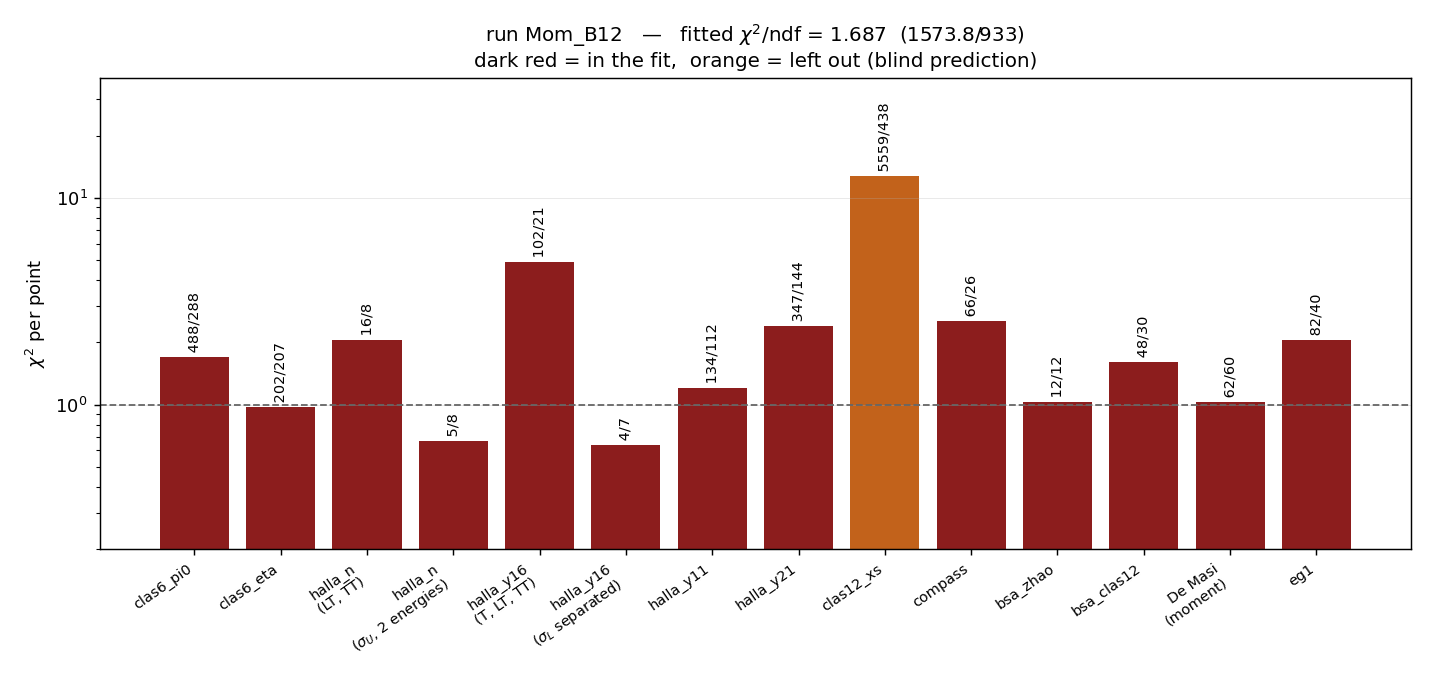
\includegraphics[width=\textwidth]{00_chi2_summary.png}
\caption{All fourteen sets at a glance: $\chi^2$ per point, fitted and blind.}
\end{figure}

\begin{figure}[p]\centering
\includegraphics[width=\textwidth]{02_clas6_pi0_in_U.png}
\caption{CLAS6 $\pi^0$, $\sig{U} = \sig{T} + \epsilon\sig{L}$, with
re-computed radiative corrections.}
\end{figure}

\begin{figure}[p]\centering
\includegraphics[width=\textwidth]{02_clas6_pi0_in_LT.png}
\caption{CLAS6 $\pi^0$, $\sig{LT}$.}
\end{figure}

\begin{figure}[p]\centering
\includegraphics[width=\textwidth]{02_clas6_pi0_in_TT.png}
\caption{CLAS6 $\pi^0$, $\sig{TT}$.}
\end{figure}

\begin{figure}[p]\centering
\includegraphics[width=\textwidth]{03_clas6_eta_in_U.png}
\caption{CLAS6 $\eta$, $\sig{U}$.  This channel probes $2X_u - X_d$.}
\end{figure}

\begin{figure}[p]\centering
\includegraphics[width=\textwidth]{03_clas6_eta_in_LT.png}
\caption{CLAS6 $\eta$, $\sig{LT}$.}
\end{figure}

\begin{figure}[p]\centering
\includegraphics[width=\textwidth]{03_clas6_eta_in_TT.png}
\caption{CLAS6 $\eta$, $\sig{TT}$.}
\end{figure}

\begin{figure}[p]\centering
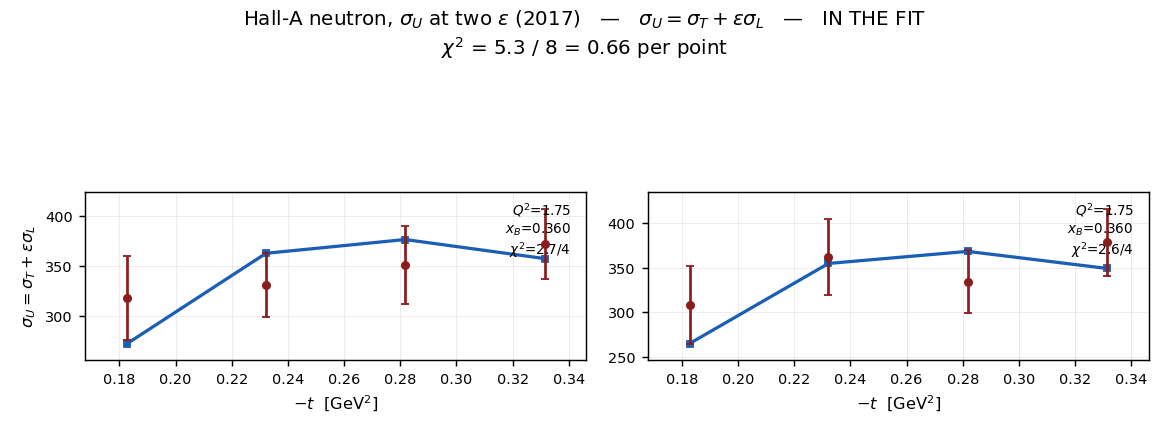
\includegraphics[width=0.8\textwidth]{05_halla_n_U_in_U.png}
\caption{Hall A neutron, $\sig{U}$ at the two beam energies.  Recovered from
PRL~\textbf{118} 222002, section~\ref{sec:recovered}; these eight points
replace the four derived $\sig{T}$.}
\end{figure}

\begin{figure}[p]\centering
\includegraphics[width=0.8\textwidth]{04_halla_n_in_LT.png}
\includegraphics[width=0.8\textwidth]{04_halla_n_in_TT.png}
\caption{Hall A neutron, $\sig{LT}$ and $\sig{TT}$, published values.}
\end{figure}

\begin{figure}[p]\centering
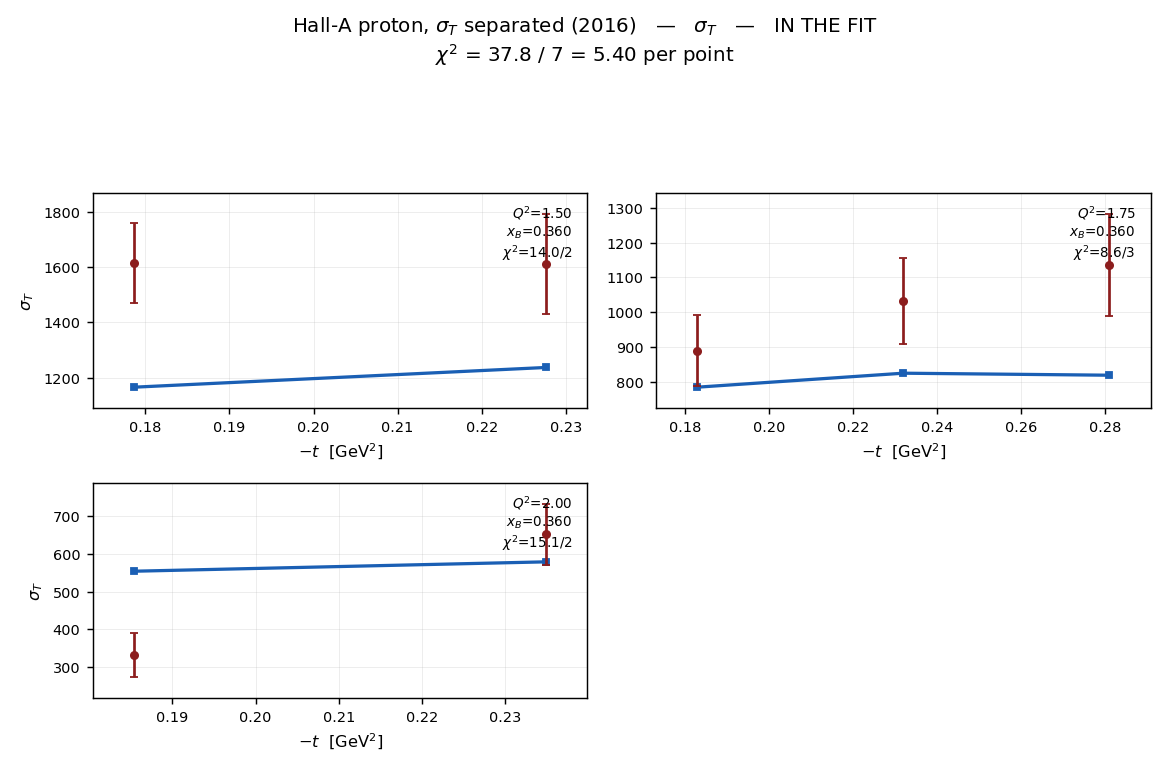
\includegraphics[width=0.8\textwidth]{06_halla_y16_in_T.png}
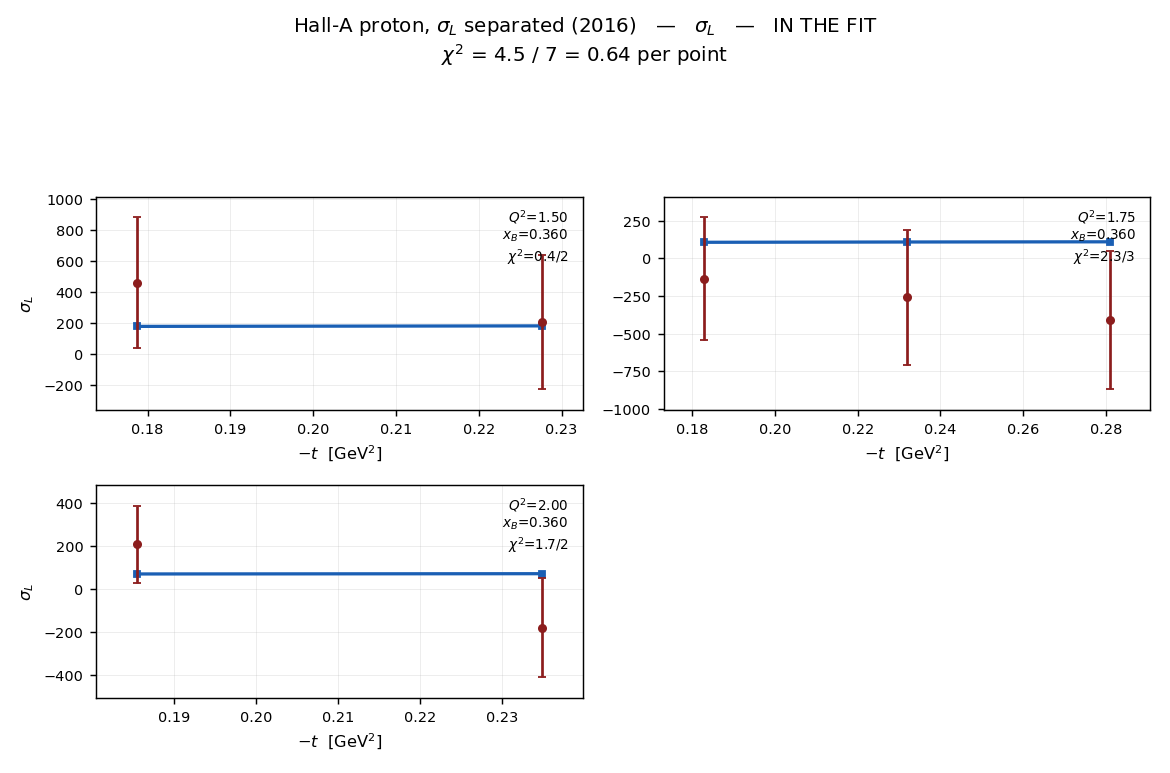
\includegraphics[width=0.8\textwidth]{07_halla_y16_L_in_L.png}
\caption{Hall A 2016, the Rosenbluth separation.  $\sig{T}$ above;
$\sig{L}$ below, recovered from the publication and absent from every fit
before October 2026.  Note the vertical scale of the lower panel: the errors
are of the size of the values.}
\end{figure}

\begin{figure}[p]\centering
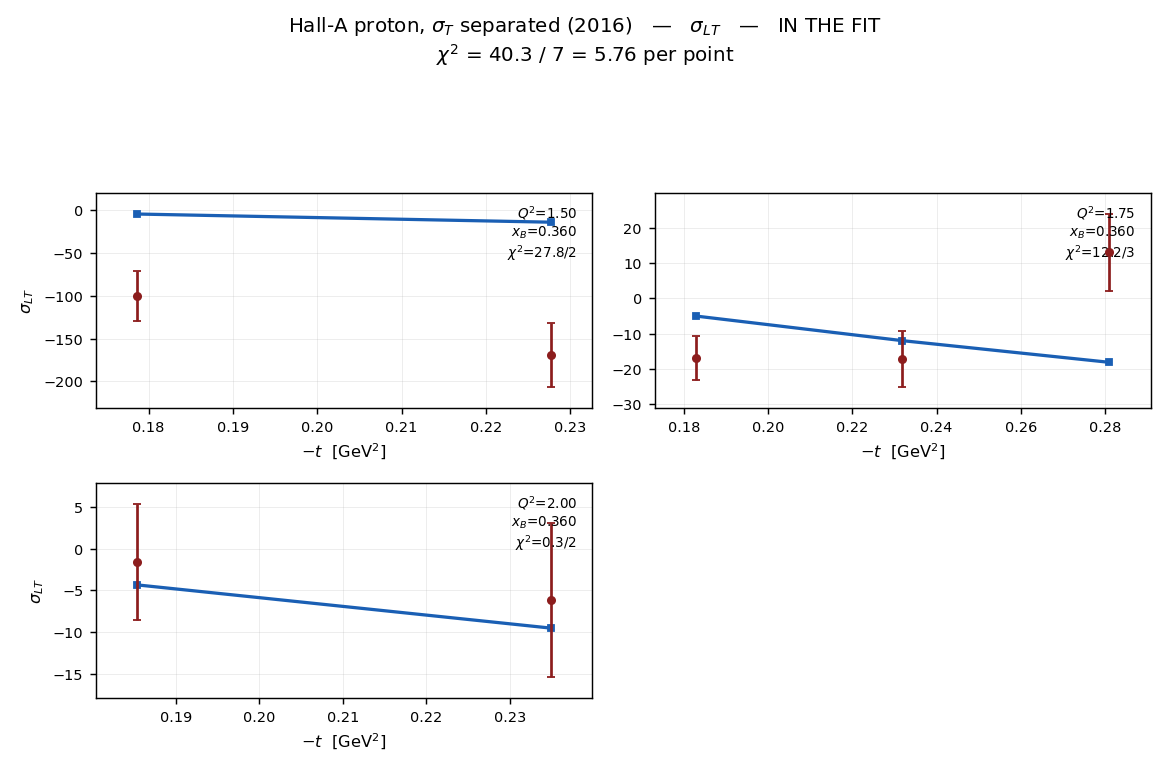
\includegraphics[width=0.8\textwidth]{06_halla_y16_in_LT.png}
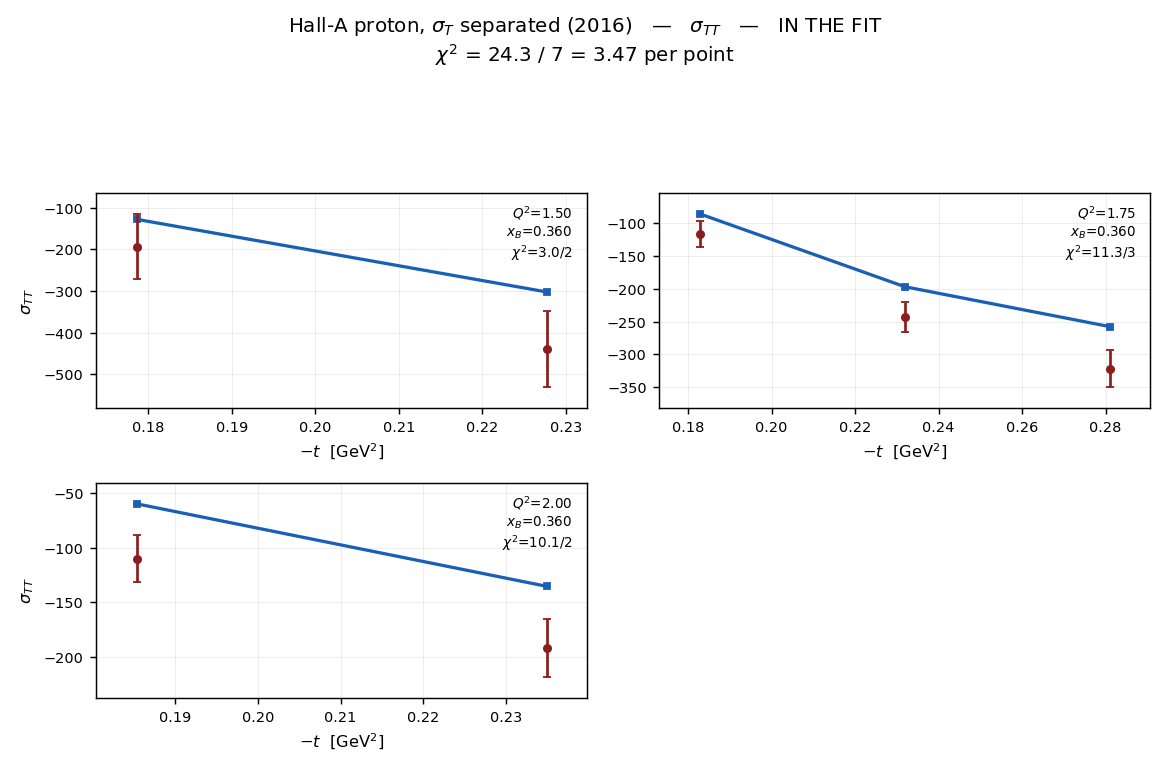
\includegraphics[width=0.8\textwidth]{06_halla_y16_in_TT.png}
\caption{Hall A 2016, $\sig{LT}$ and $\sig{TT}$.  The two $Q^2 = 1.50$ points
of the upper panel are two of the three that no smooth model reaches,
section~\ref{sec:sigmalt}.}
\end{figure}

\begin{figure}[p]\centering
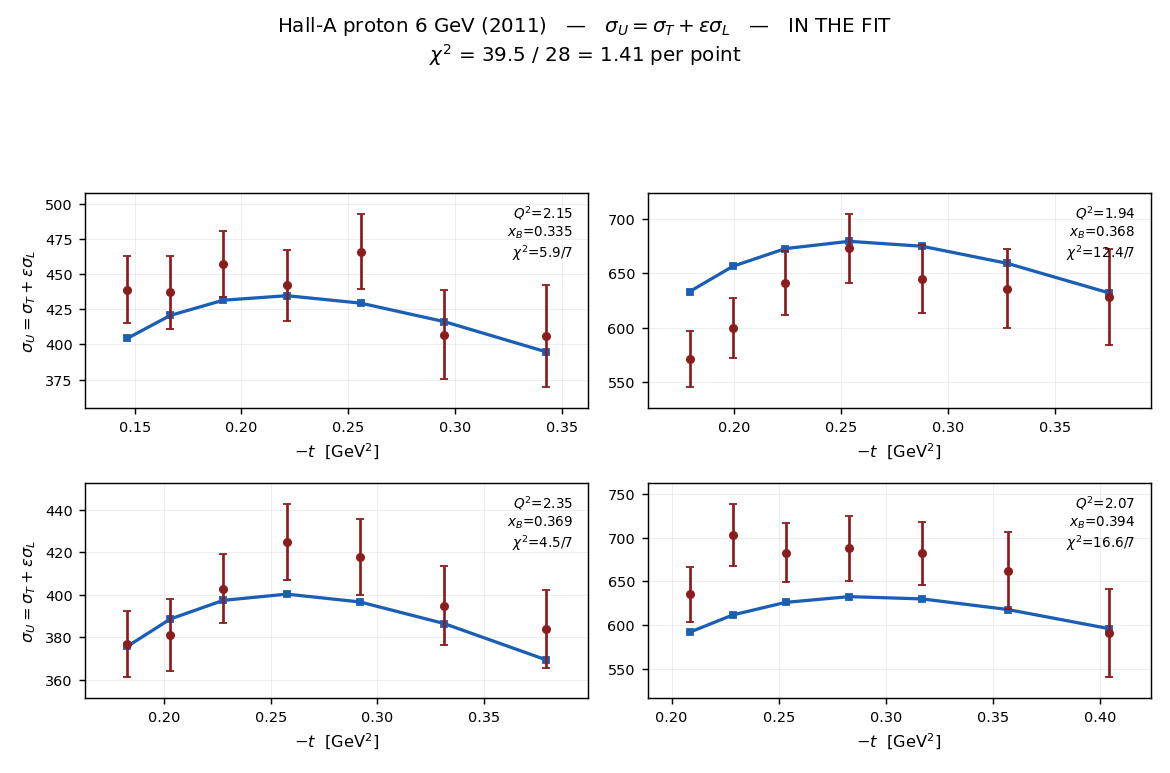
\includegraphics[width=\textwidth]{08_halla_y11_in_U.png}
\caption{Hall A 2011, $\sig{U}$.}
\end{figure}

\begin{figure}[p]\centering
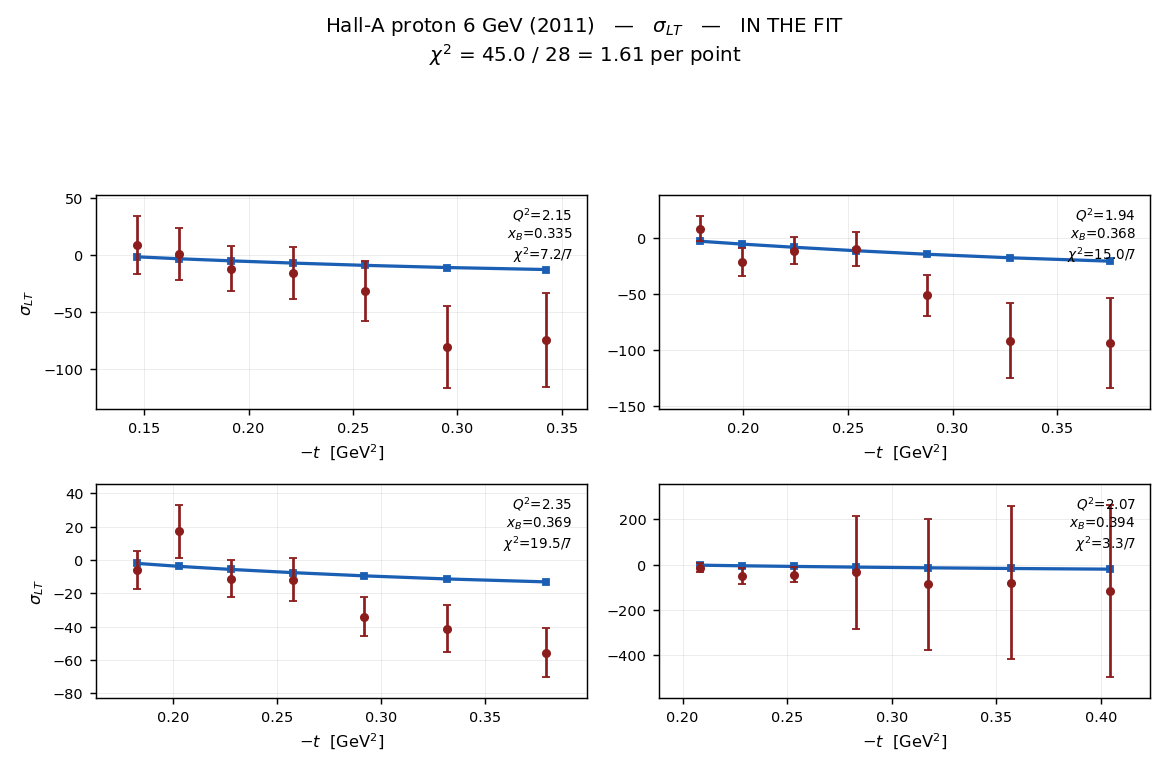
\includegraphics[width=\textwidth]{08_halla_y11_in_LT.png}
\caption{Hall A 2011, $\sig{LT}$.}
\end{figure}

\begin{figure}[p]\centering
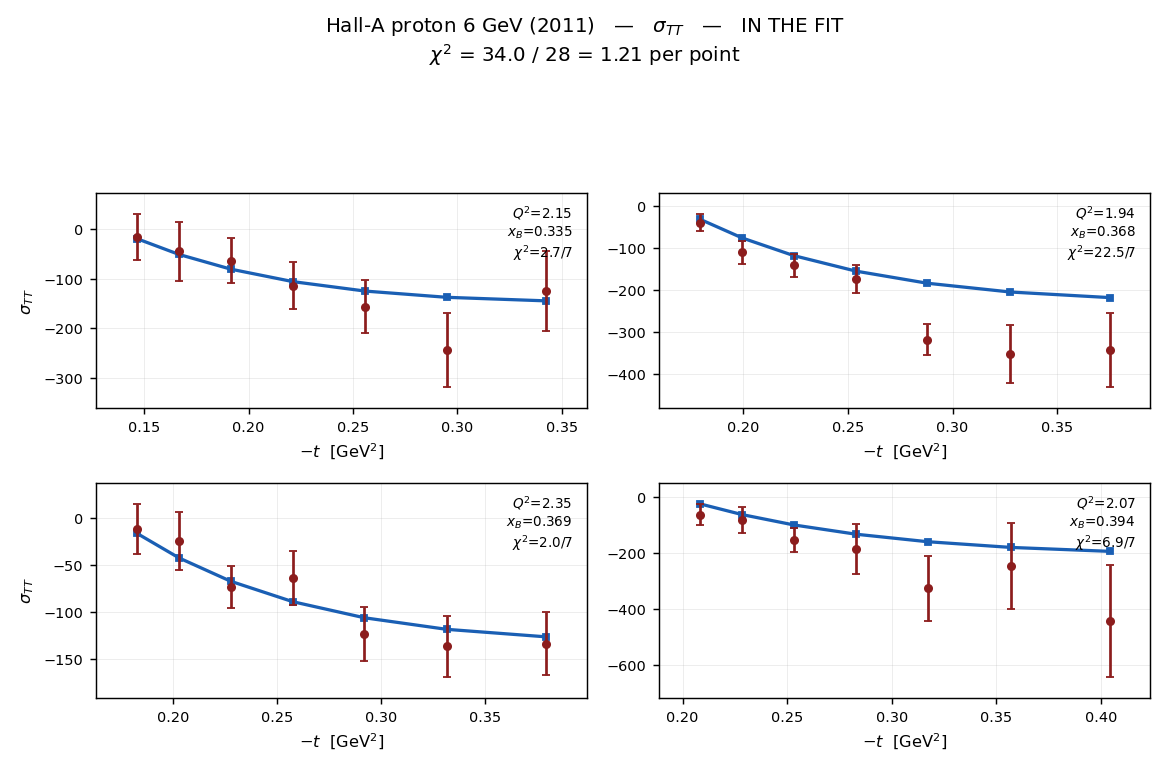
\includegraphics[width=\textwidth]{08_halla_y11_in_TT.png}
\caption{Hall A 2011, $\sig{TT}$.}
\end{figure}

\begin{figure}[p]\centering
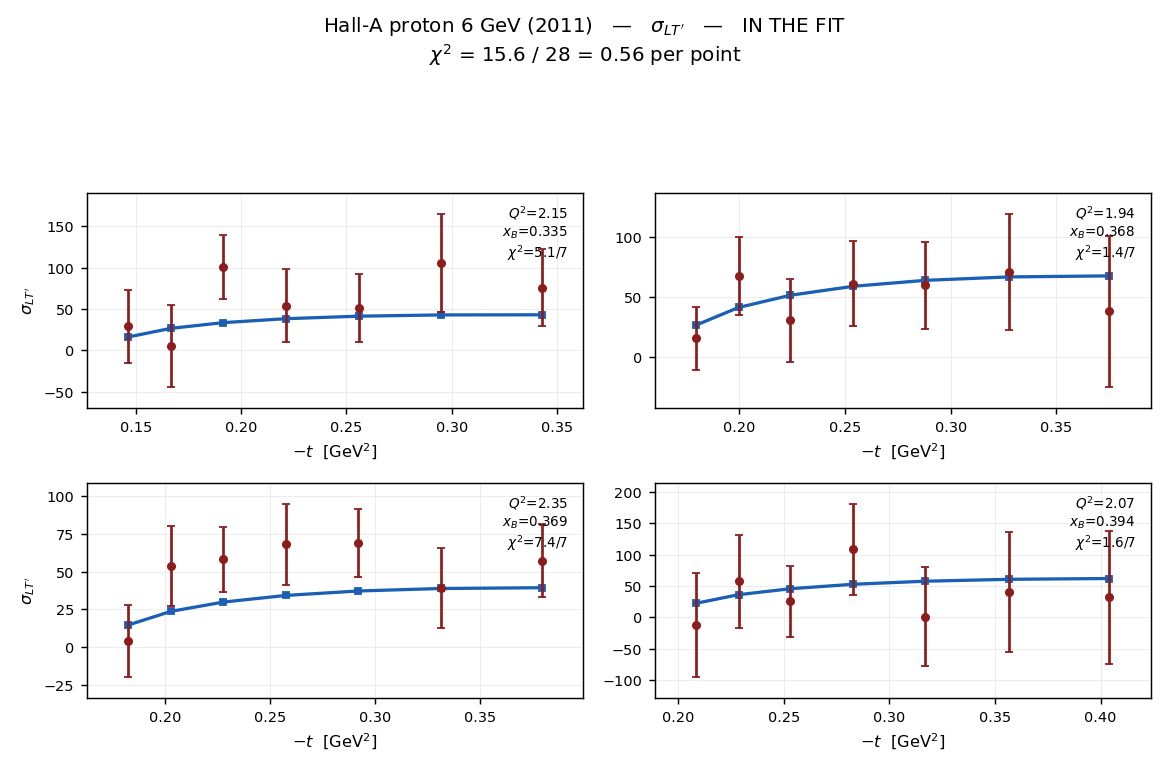
\includegraphics[width=\textwidth]{08_halla_y11_in_LTp.png}
\caption{Hall A 2011, $\sig{LT'}$ --- one of the two direct measurements of the
quantity that section~\ref{sec:sigmaltp} finds too small in the model.}
\end{figure}

\begin{figure}[p]\centering
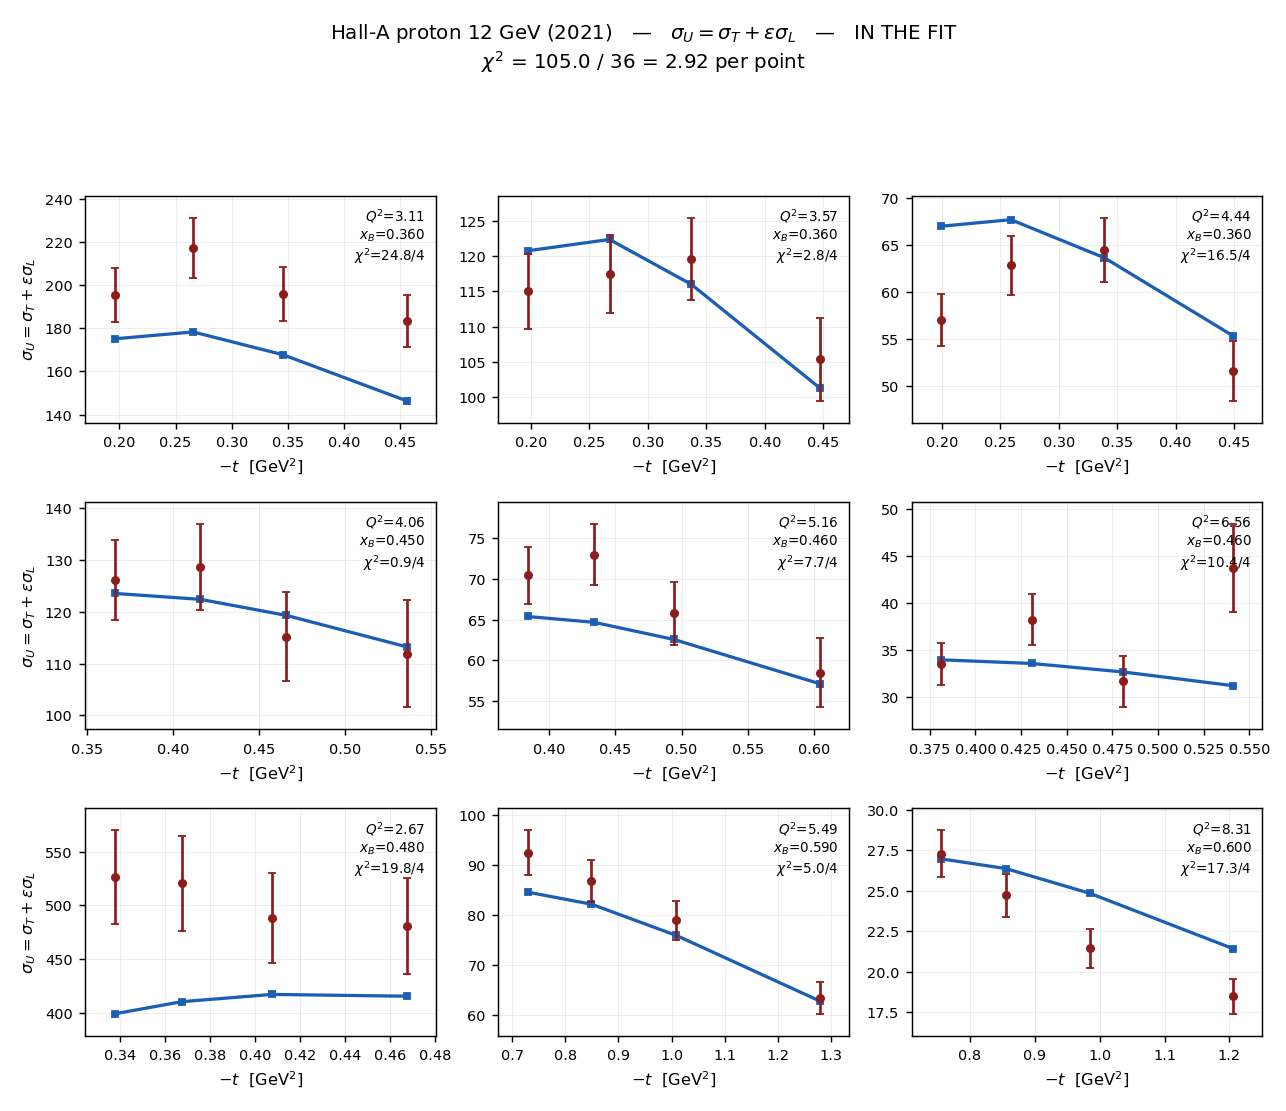
\includegraphics[width=\textwidth]{09_halla_y21_in_U.png}
\caption{Hall A 2021, $\sig{U}$.}
\end{figure}

\begin{figure}[p]\centering
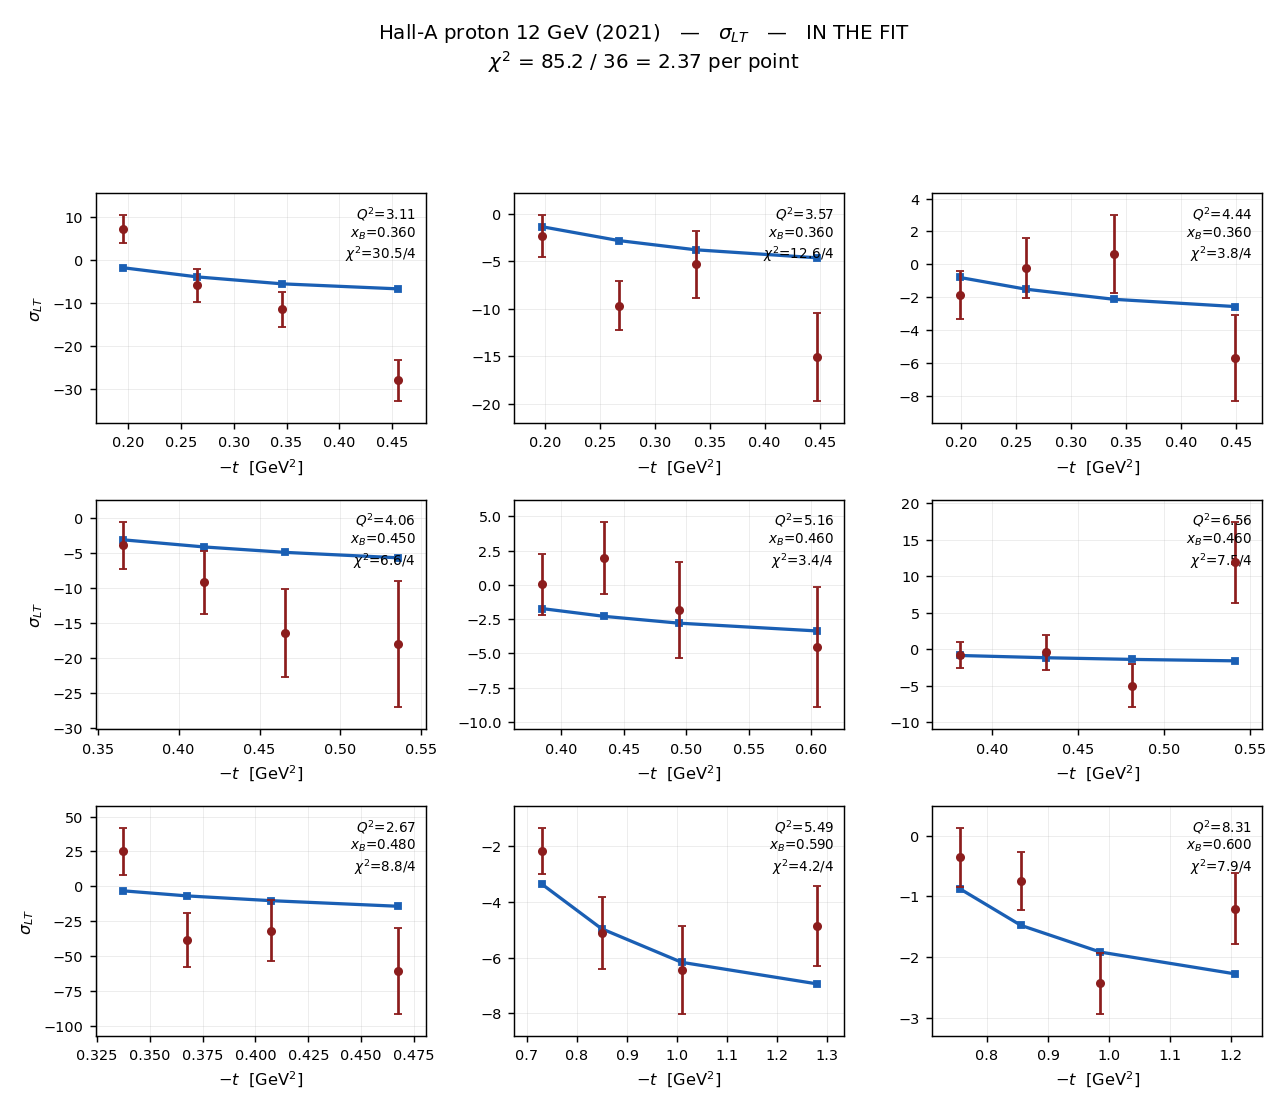
\includegraphics[width=\textwidth]{09_halla_y21_in_LT.png}
\caption{Hall A 2021, $\sig{LT}$.}
\end{figure}

\begin{figure}[p]\centering
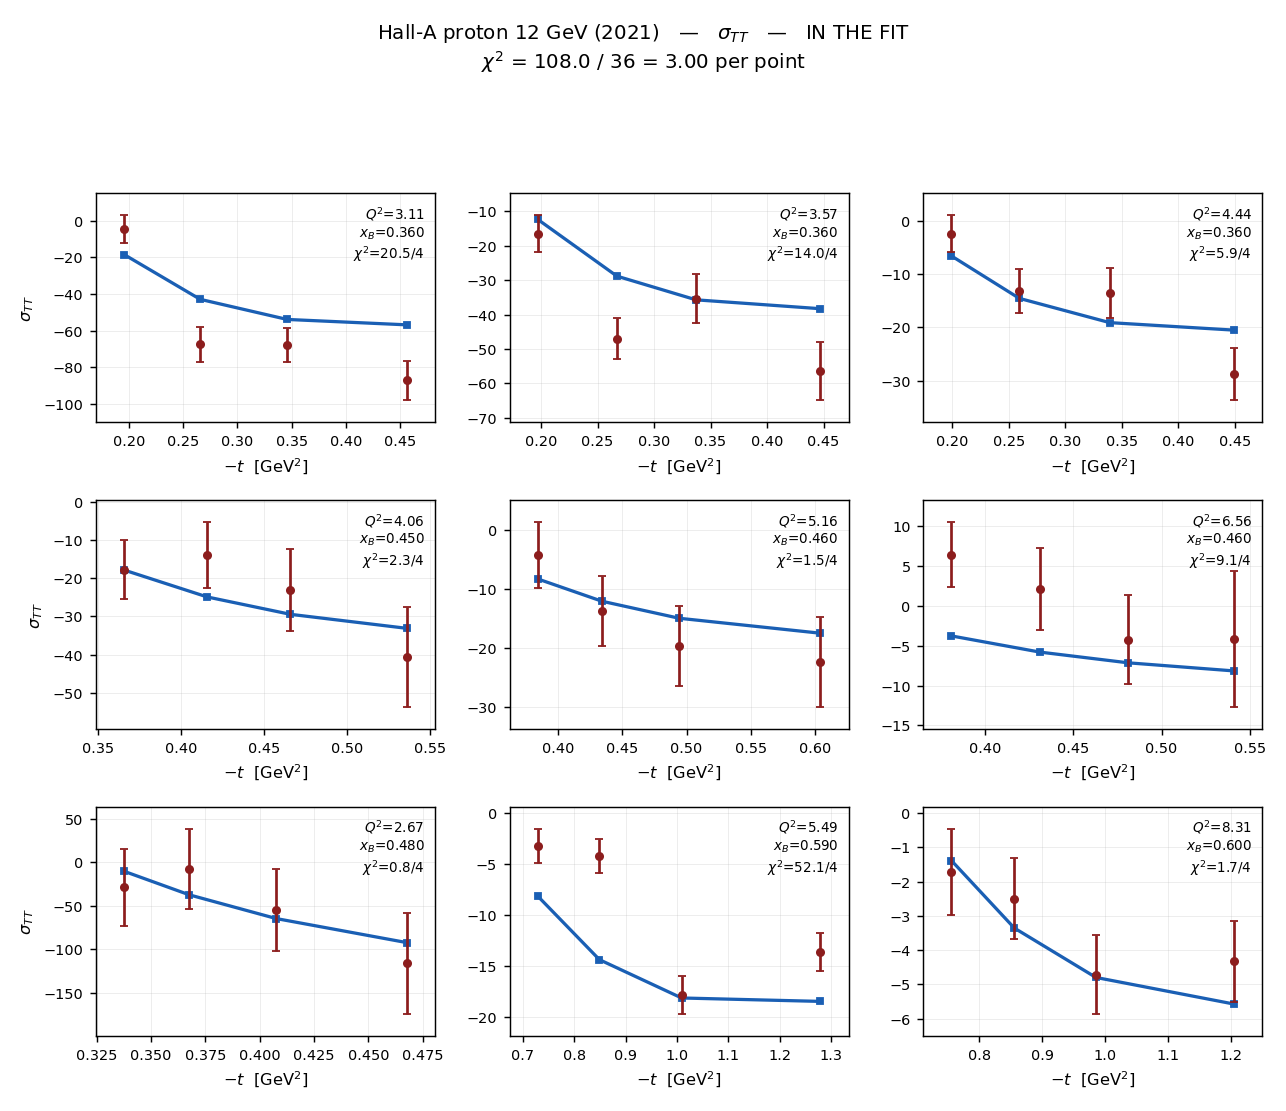
\includegraphics[width=\textwidth]{09_halla_y21_in_TT.png}
\caption{Hall A 2021, $\sig{TT}$.}
\end{figure}

\begin{figure}[p]\centering
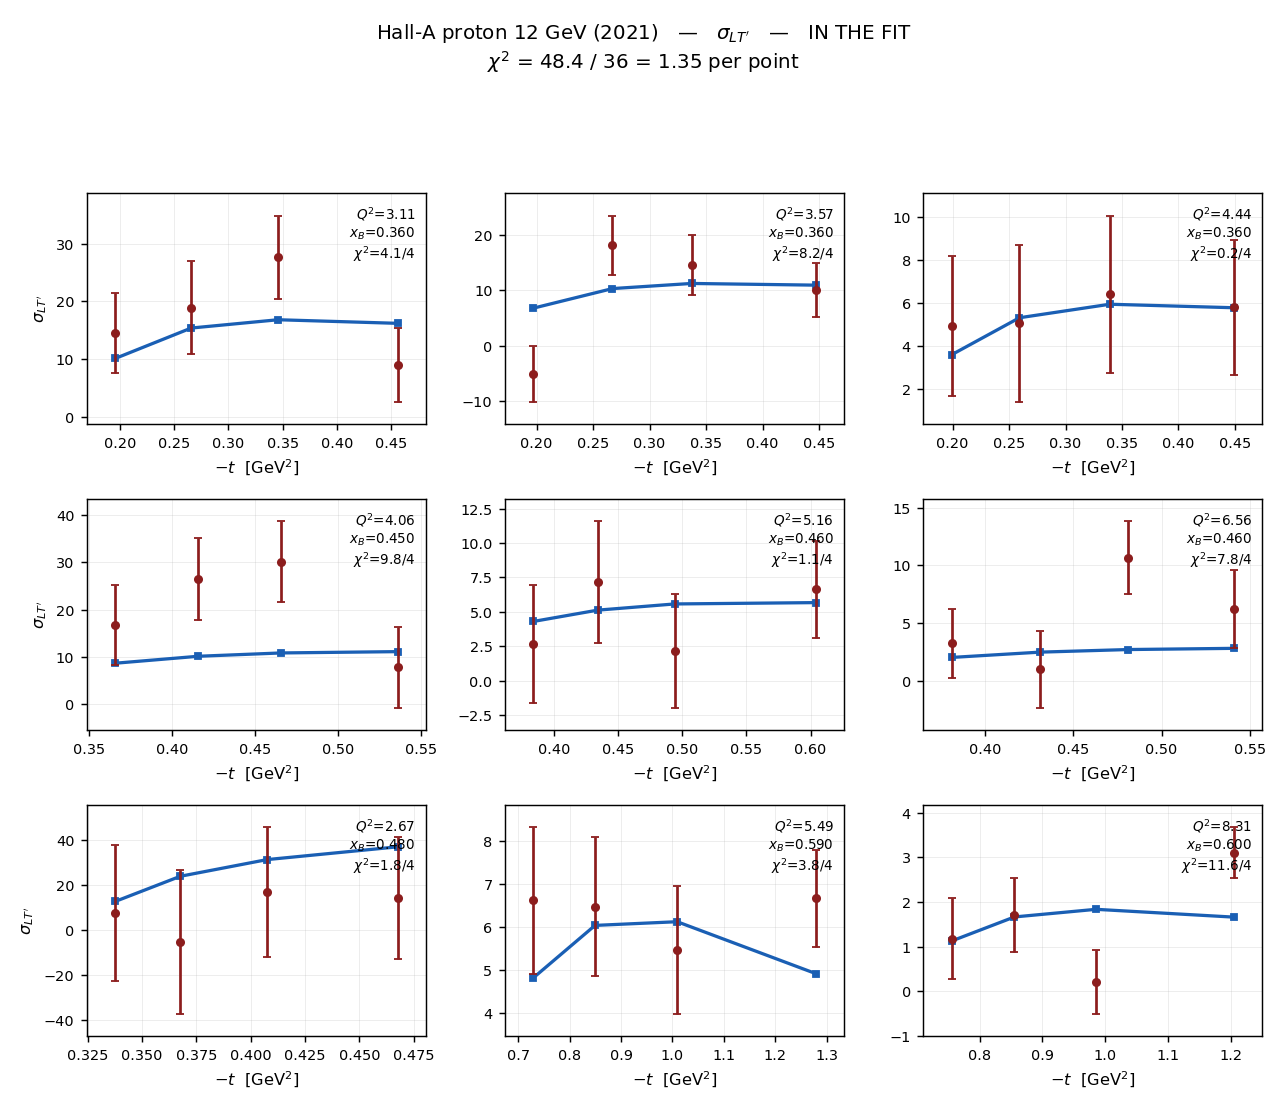
\includegraphics[width=\textwidth]{09_halla_y21_in_LTp.png}
\caption{Hall A 2021, $\sig{LT'}$.}
\end{figure}

\begin{figure}[p]\centering
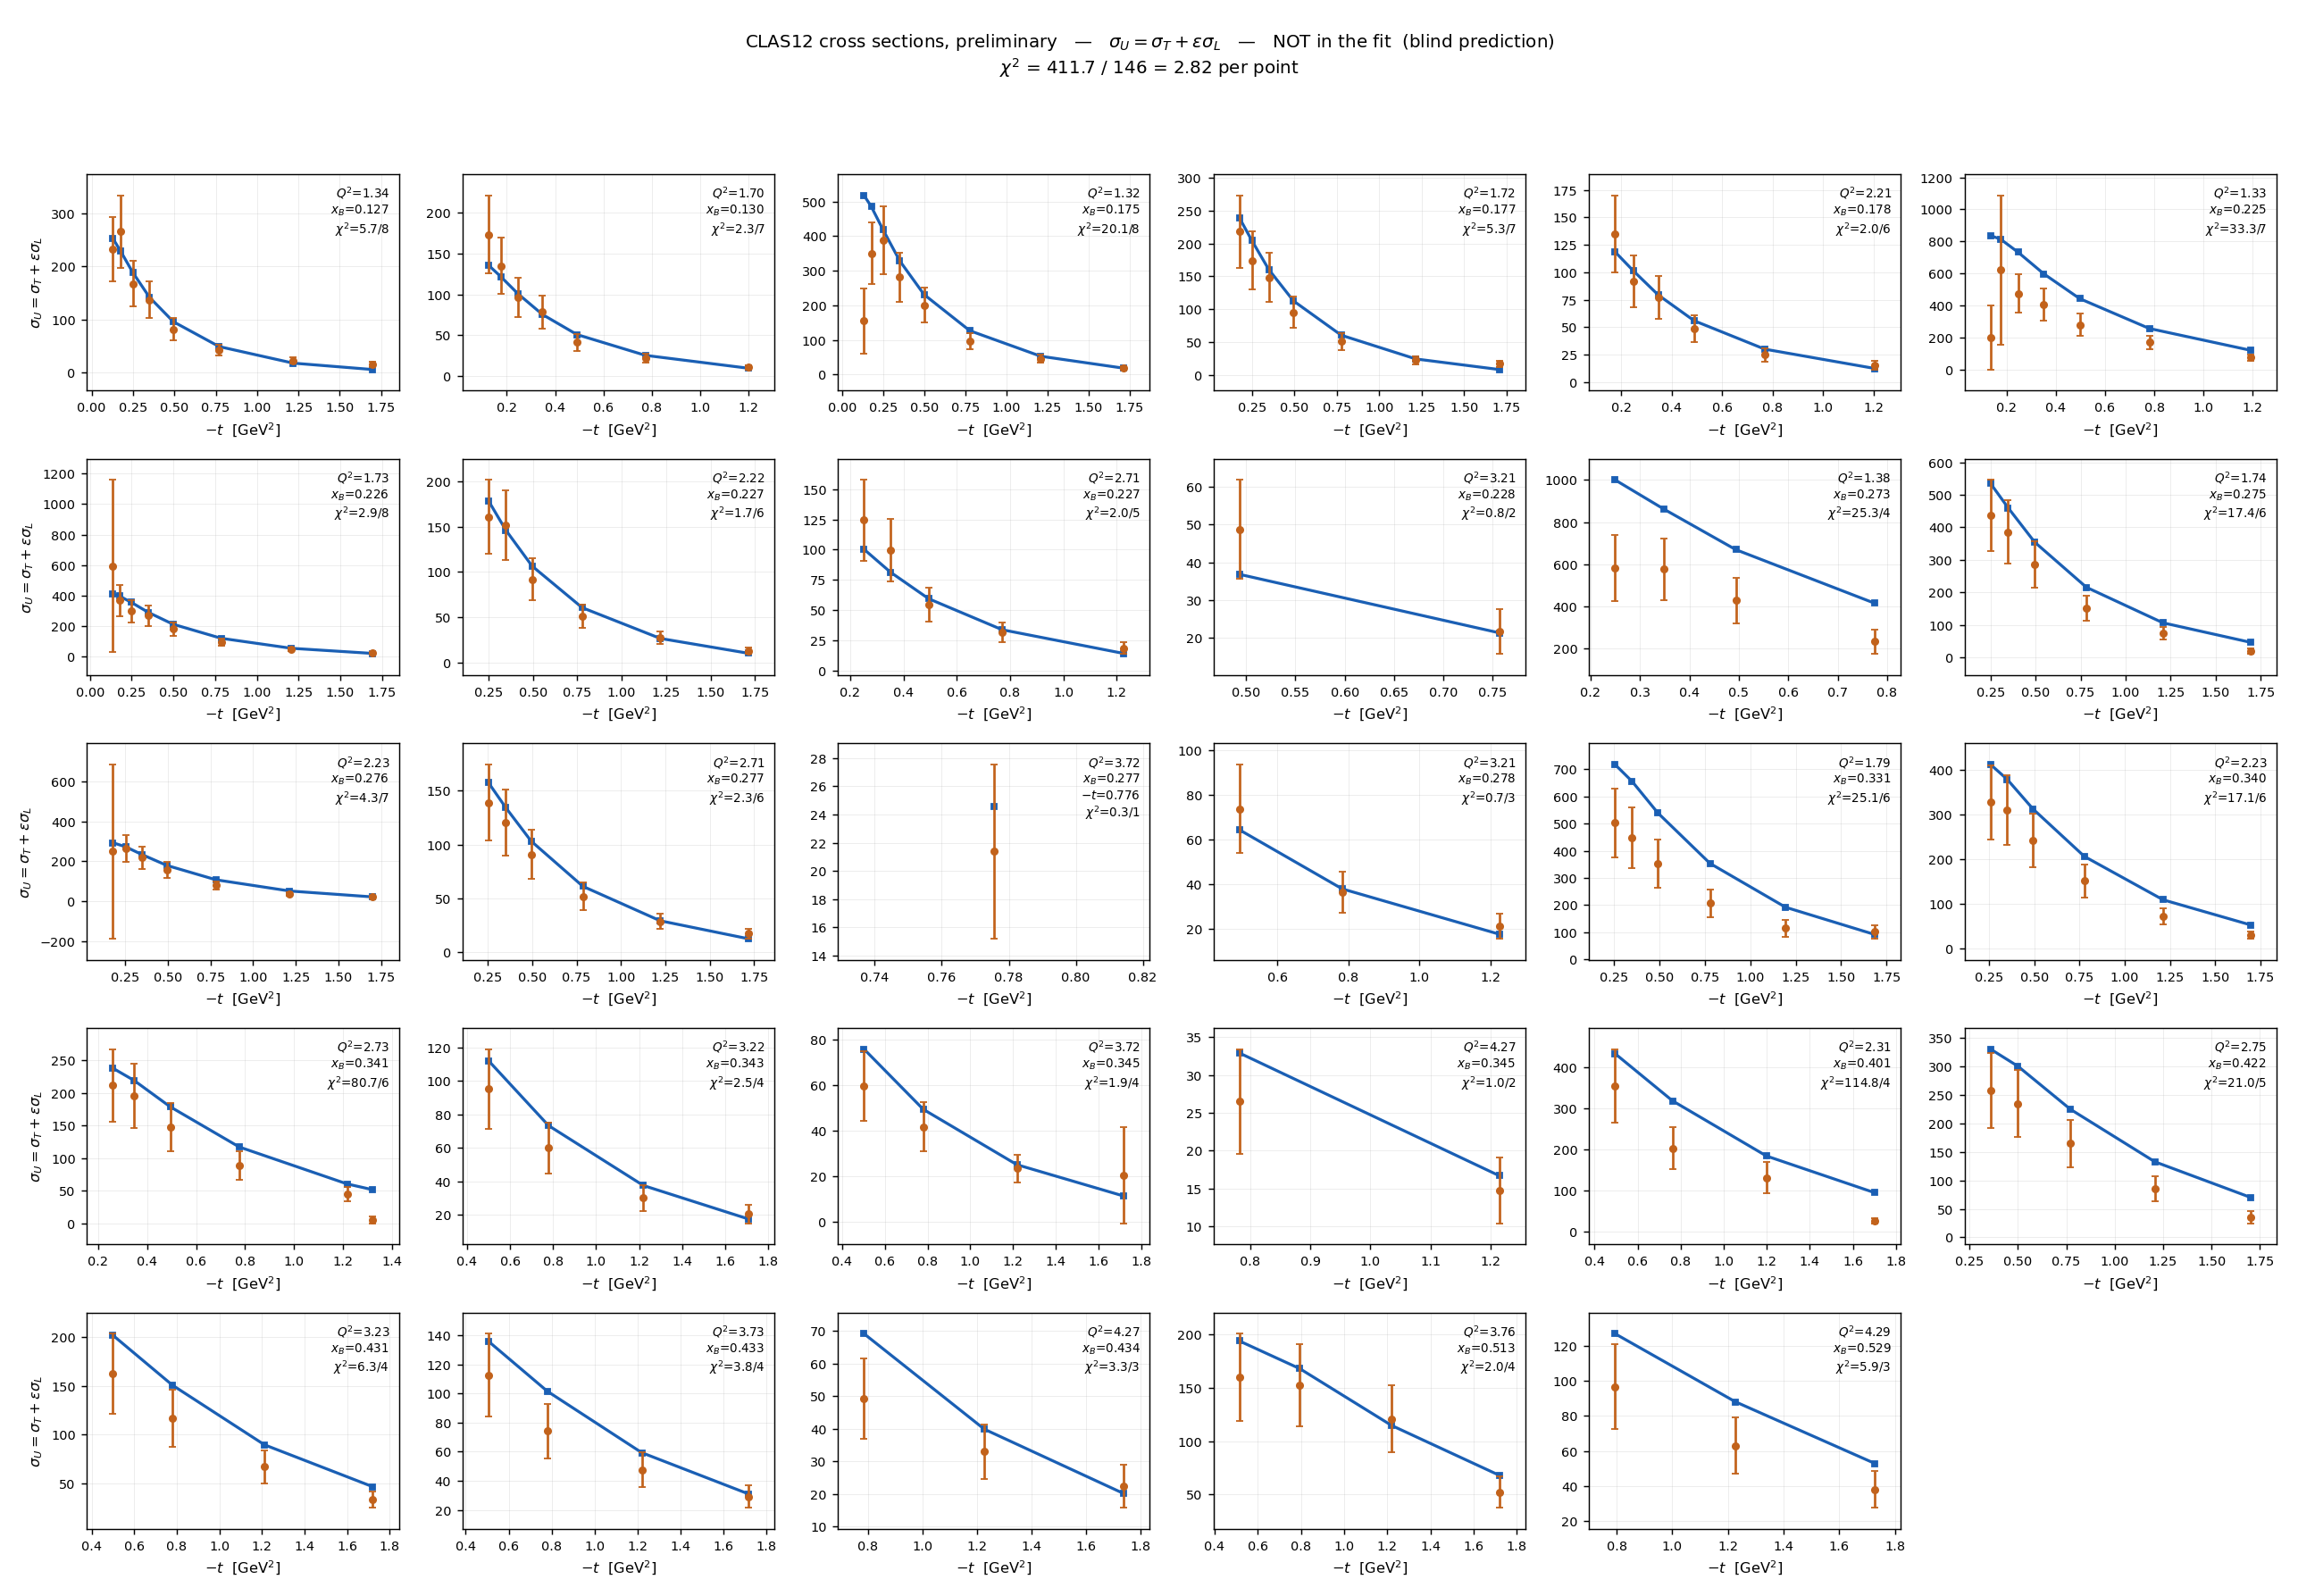
\includegraphics[width=\textwidth]{10_clas12_xs_out_U.png}
\caption{CLAS12 cross sections, $\sig{U}$ --- \textsc{not in the fit}.}
\end{figure}

\begin{figure}[p]\centering
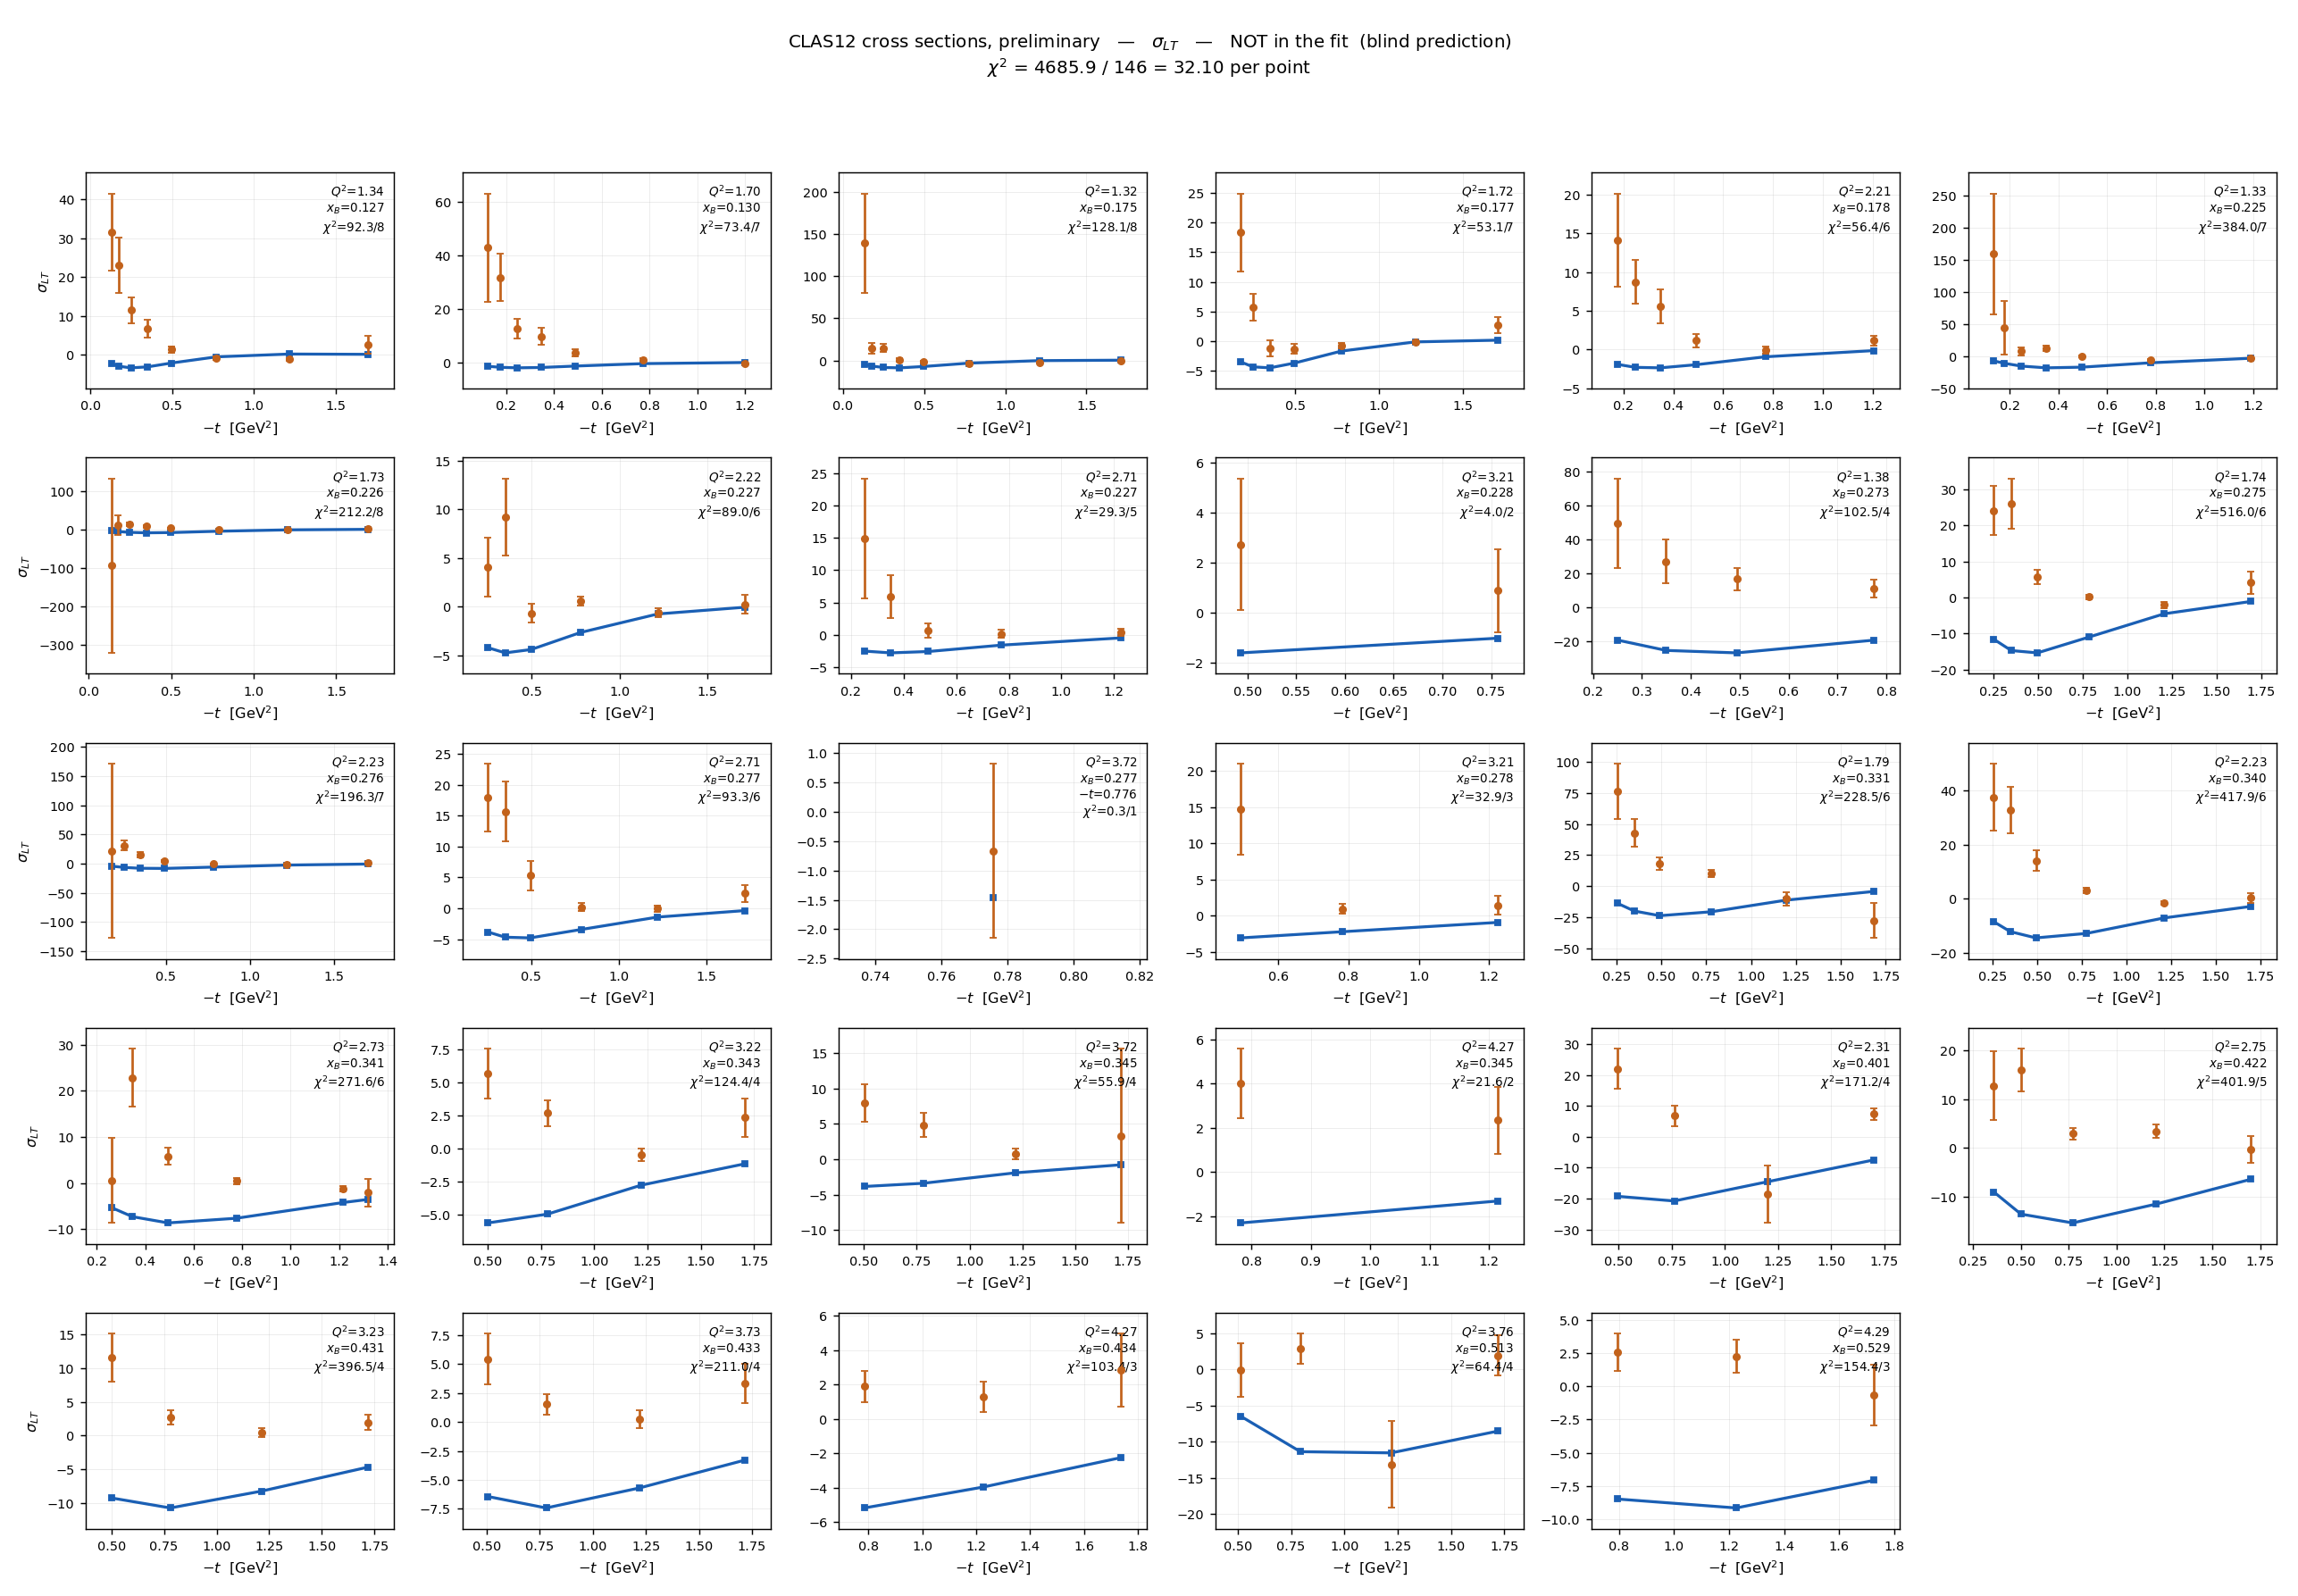
\includegraphics[width=\textwidth]{10_clas12_xs_out_LT.png}
\caption{CLAS12, $\sig{LT}$ --- \textsc{not in the fit}.  This is the sign
disagreement of section~\ref{sec:notmeasured}.}
\end{figure}

\begin{figure}[p]\centering
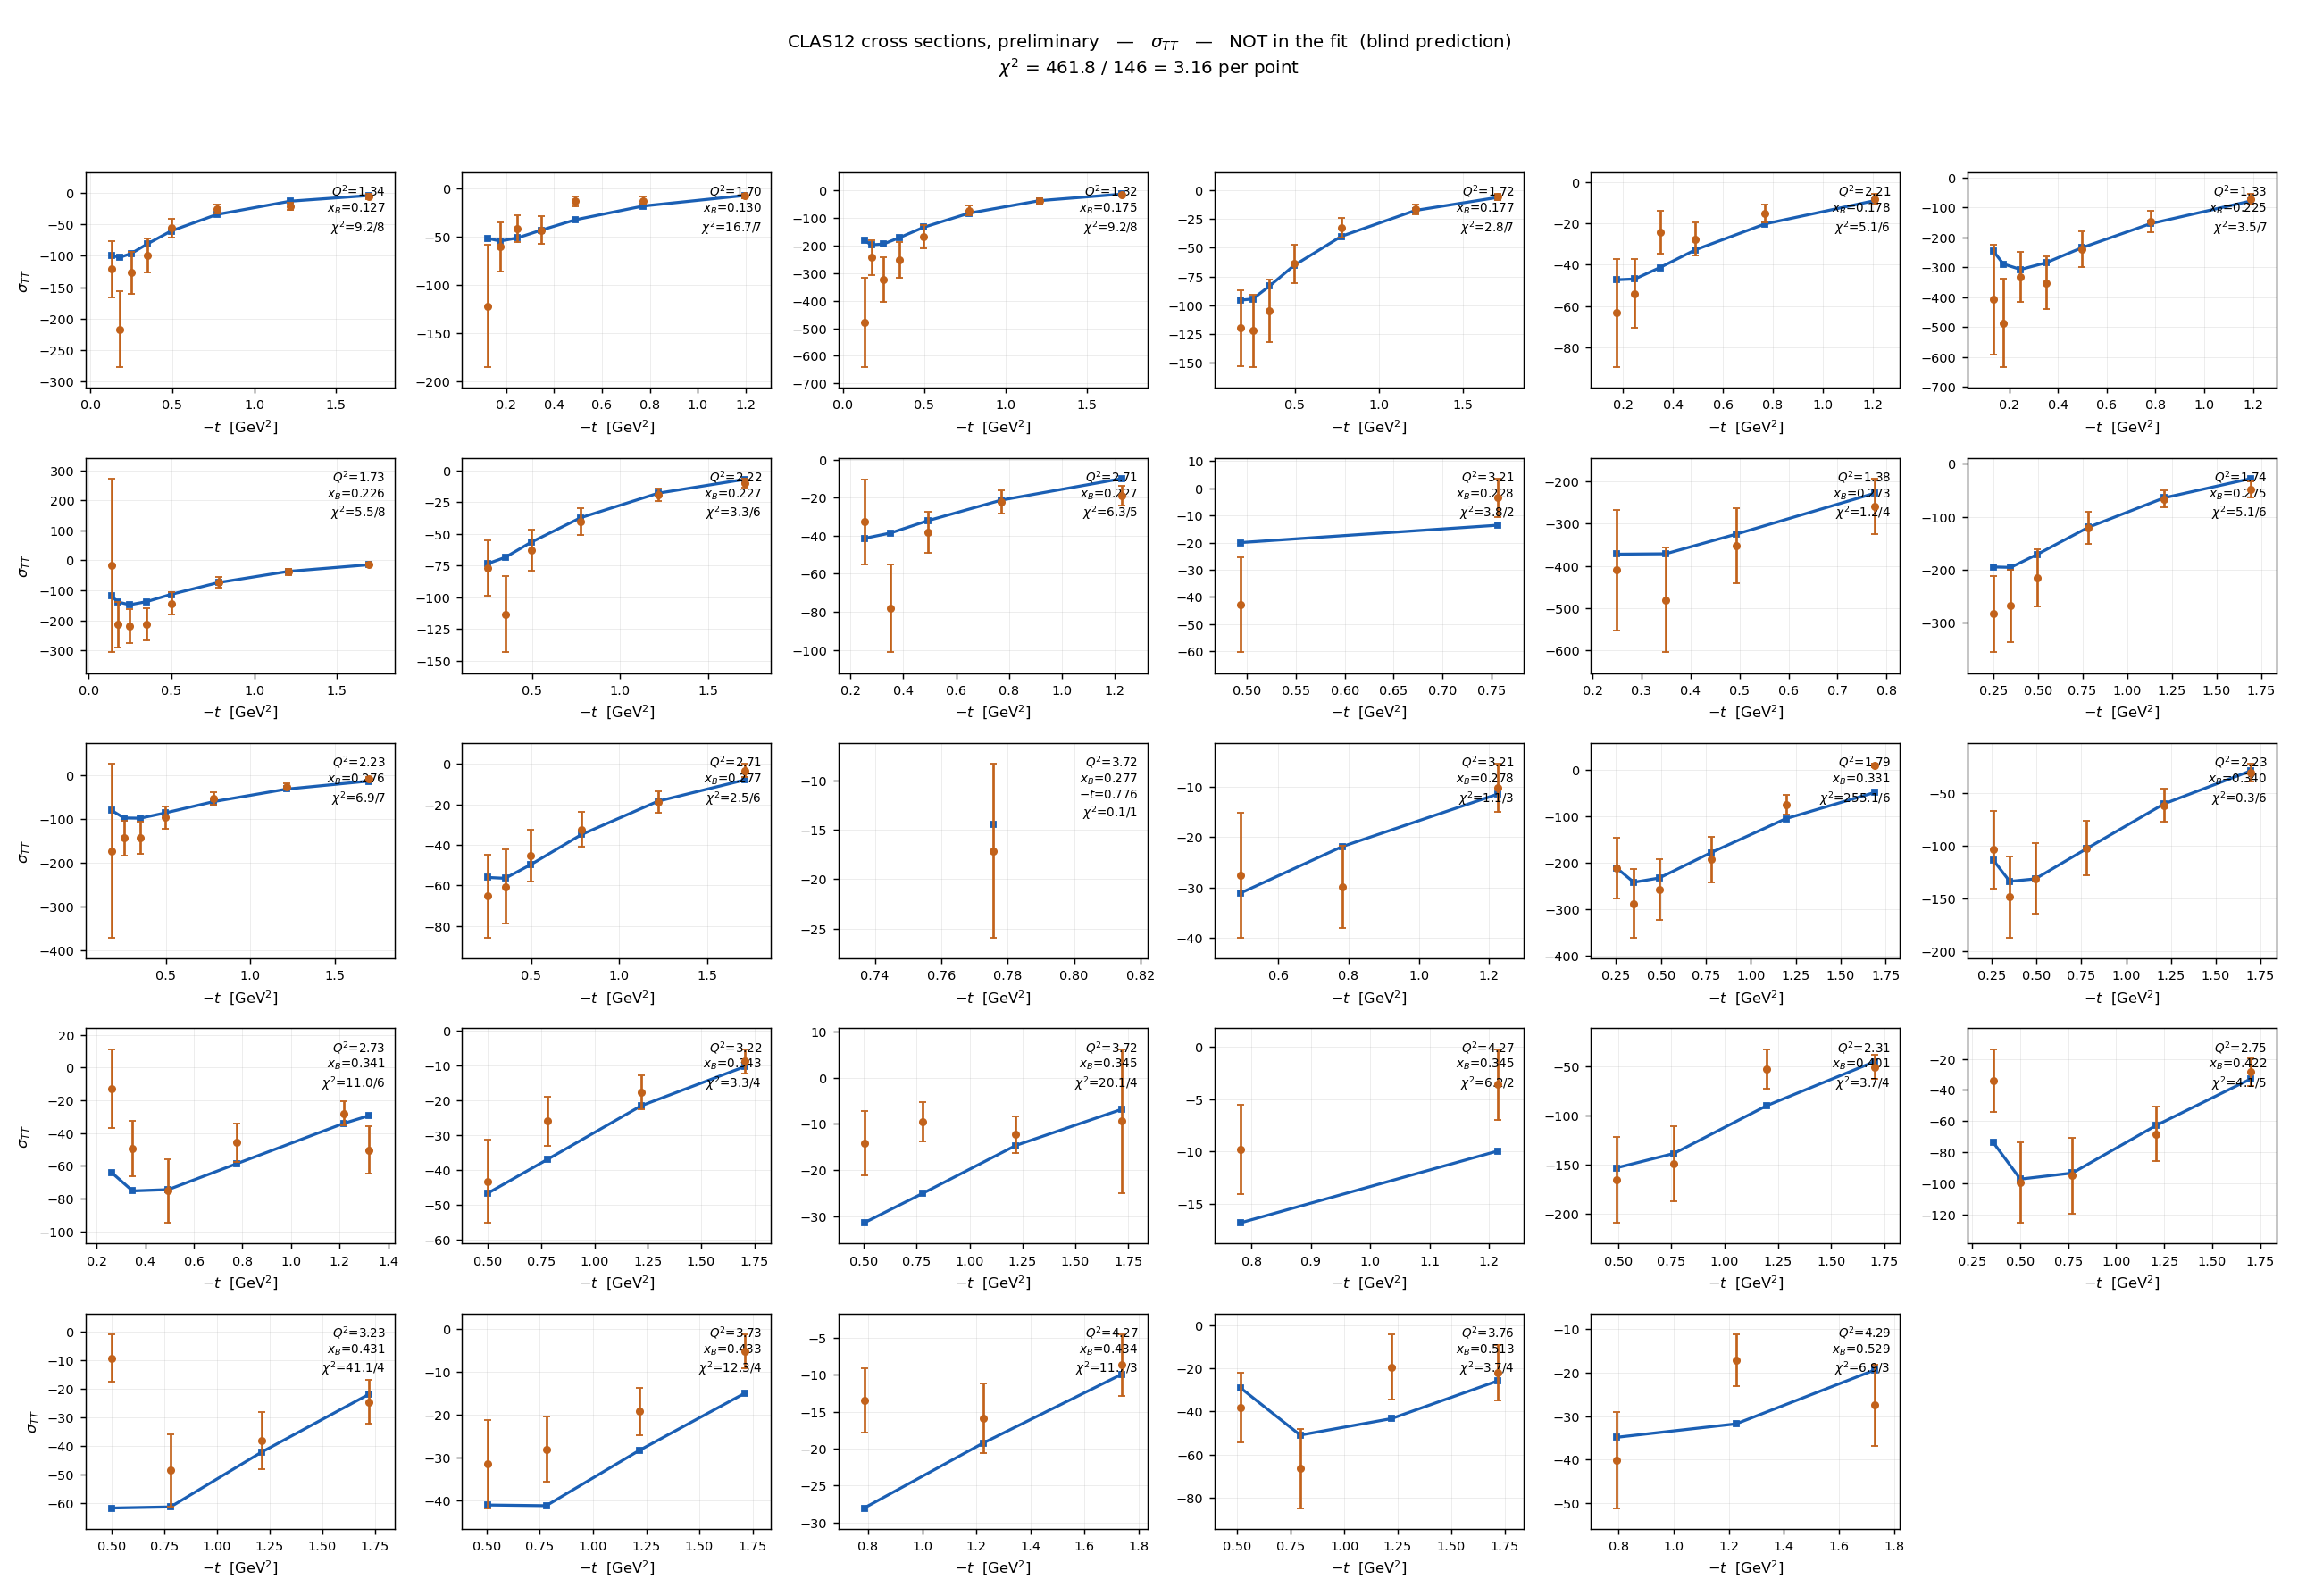
\includegraphics[width=\textwidth]{10_clas12_xs_out_TT.png}
\caption{CLAS12, $\sig{TT}$ --- \textsc{not in the fit}.}
\end{figure}

\begin{figure}[p]\centering
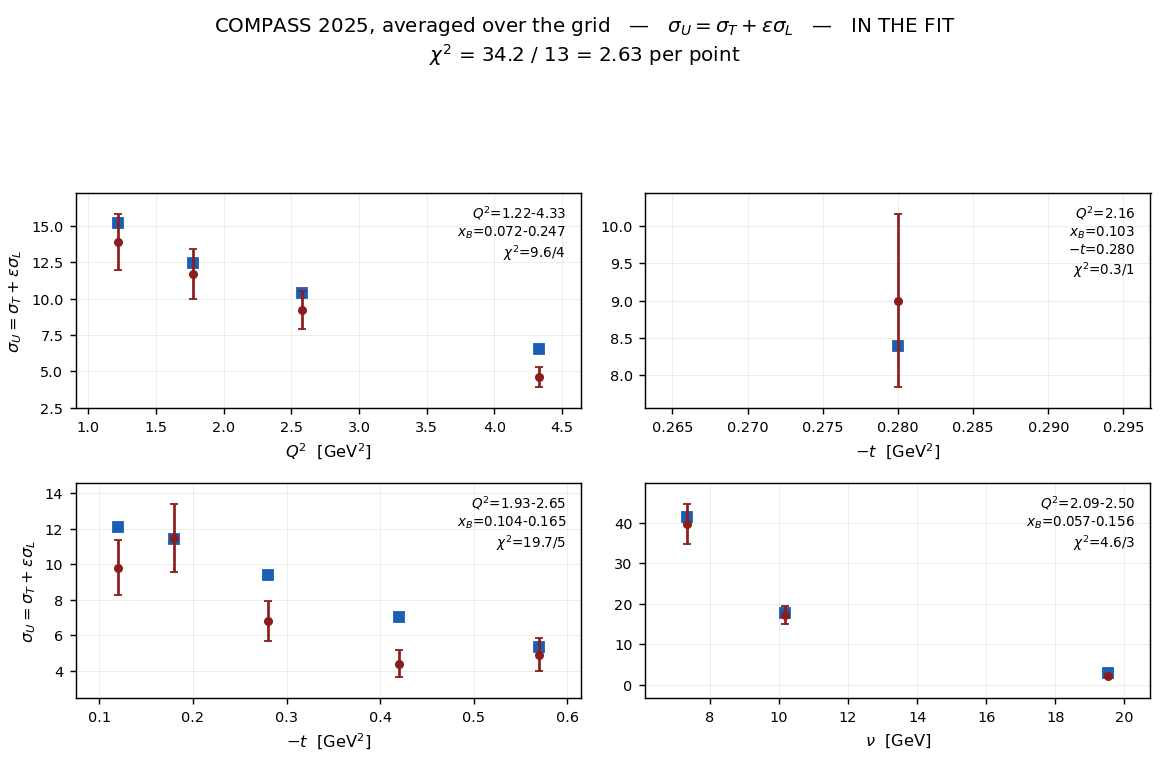
\includegraphics[width=0.8\textwidth]{11_compass_in_U.png}
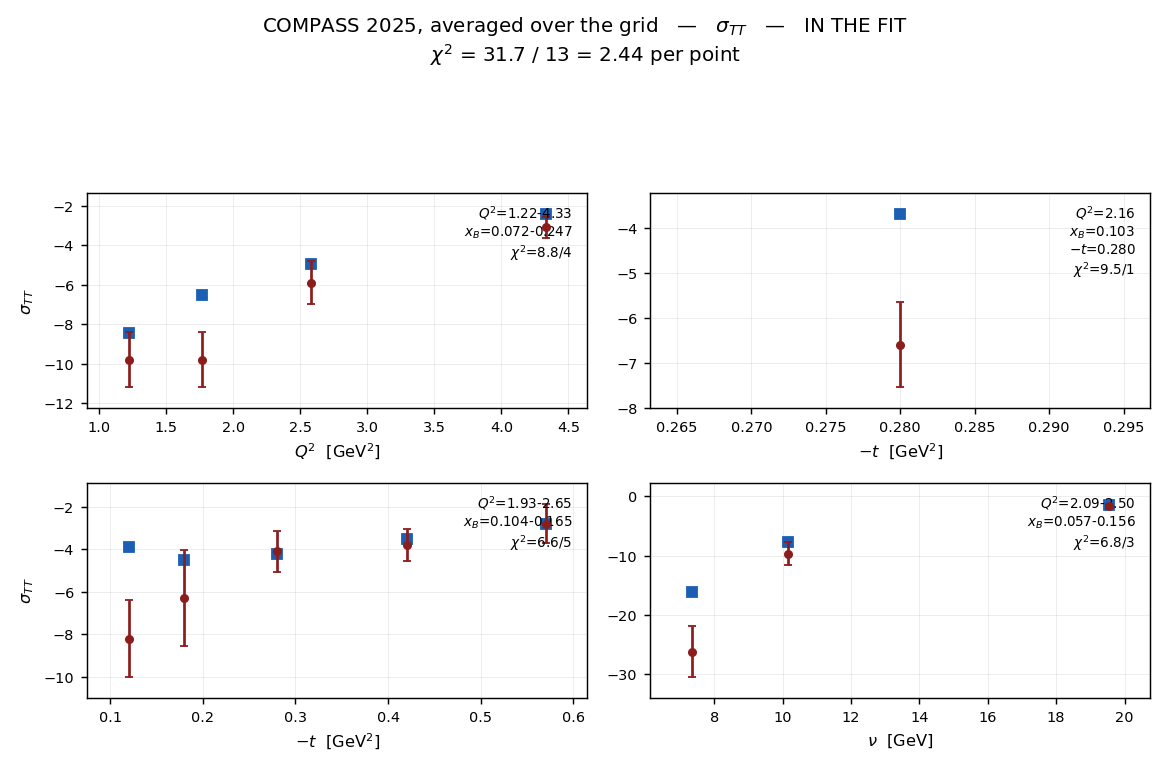
\includegraphics[width=0.8\textwidth]{11_compass_in_TT.png}
\caption{COMPASS, averaged over the published four-dimensional grid rather than
evaluated at $\langle Q^2\rangle, \langle x_B\rangle$: one cell spans $x_B$
from $0.02$ to $0.47$, and evaluating at the mean overshoots by a factor five
to eight.}
\end{figure}

\begin{figure}[p]\centering
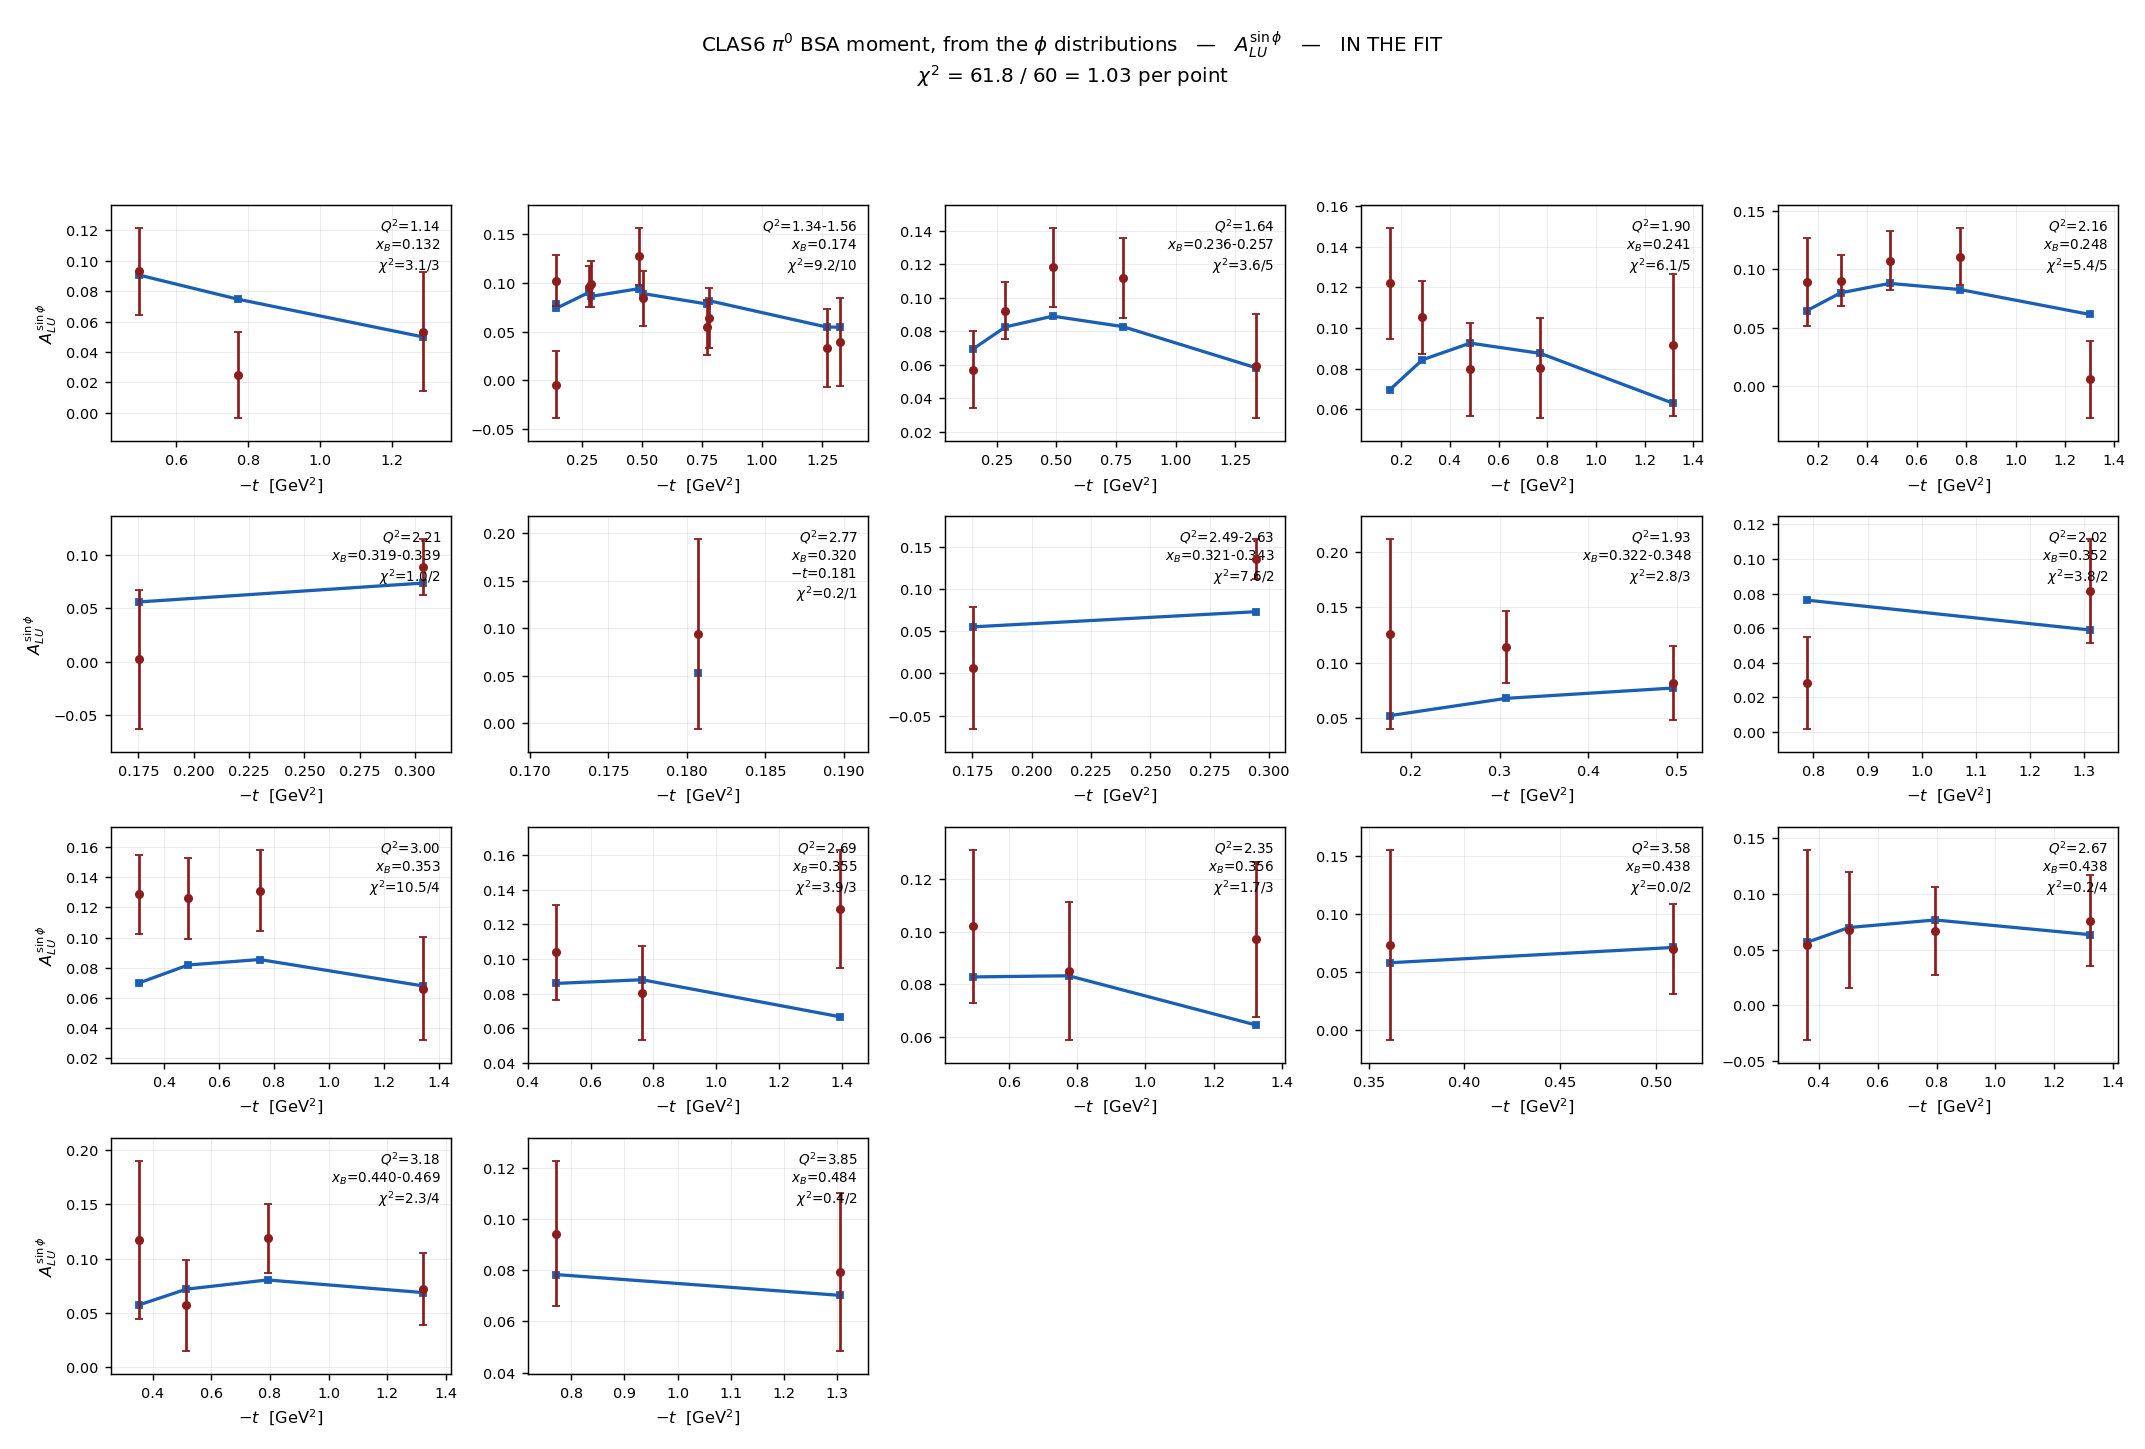
\includegraphics[width=\textwidth]{01_bsa_demasi_mom_in_A_LUsinphi.png}
\caption{De Masi, the $\sin\phi$ moment extracted from the $\phi$ distributions
with the full asymmetry form, section~\ref{sec:demasi}.}
\end{figure}


\begin{figure}[p]\centering
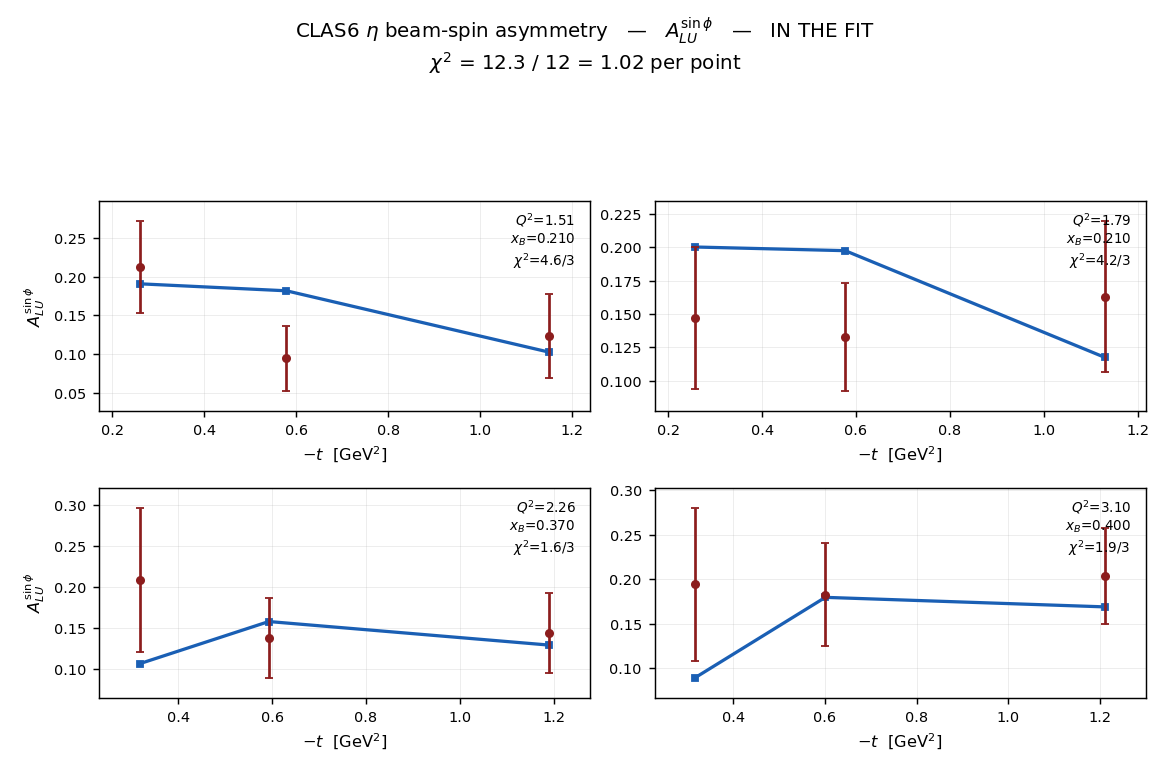
\includegraphics[width=0.8\textwidth]{13_bsa_zhao_in_A_LUsinphi.png}
\caption{Zhao, the $\eta$ beam-spin asymmetry.}
\end{figure}

\begin{figure}[p]\centering
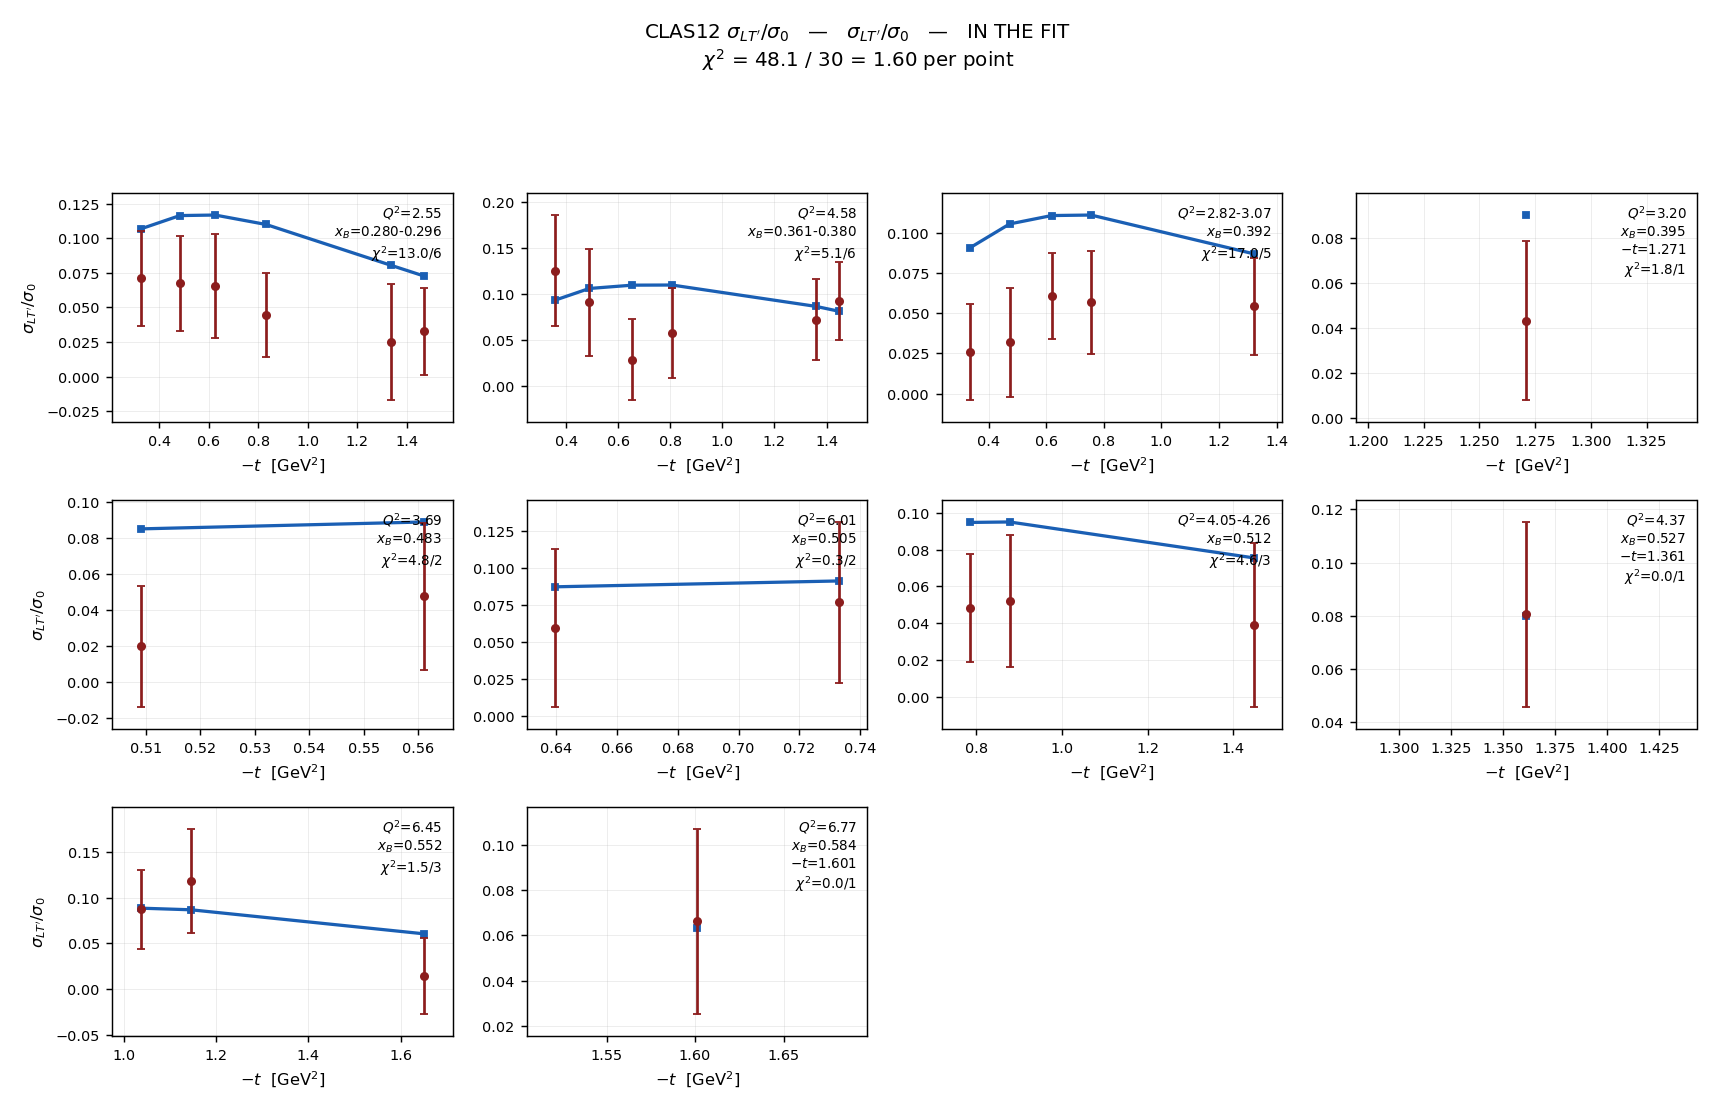
\includegraphics[width=\textwidth]{14_bsa_clas12_in_sigma_LTp_over_sigma_0.png}
\caption{CLAS12 $\sig{LT'}/\sigma_0$.}
\end{figure}

\begin{figure}[p]\centering
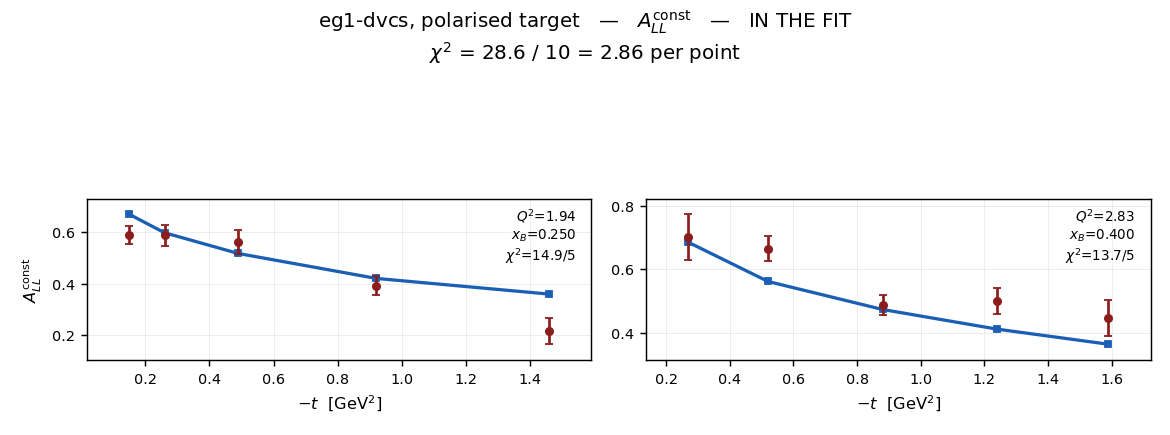
\includegraphics[width=0.72\textwidth]{15_eg1_in_ALLc.png}
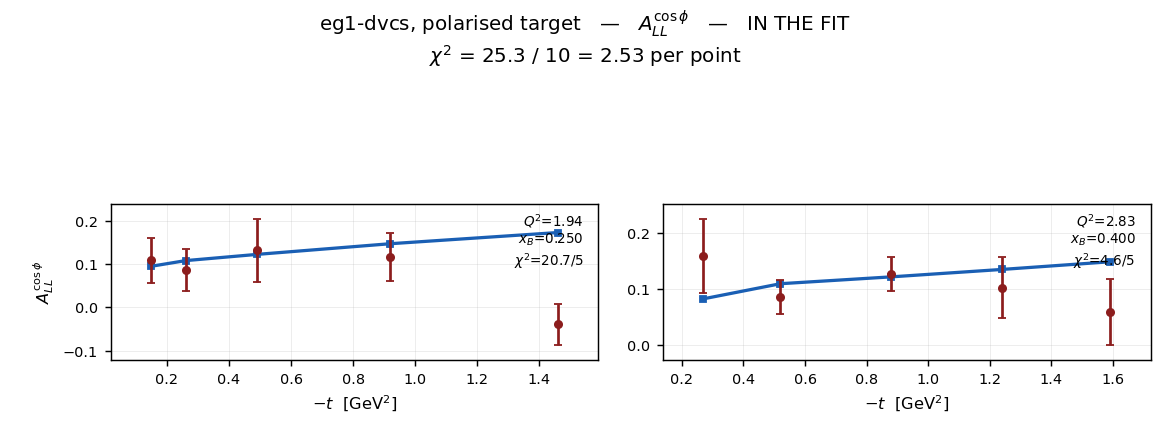
\includegraphics[width=0.72\textwidth]{15_eg1_in_ALLcos.png}
\caption{eg1-dvcs, the $A_{LL}$ moments --- the only observable in the database
that sees the $T_{01}$--$U_{01}$ relative phase.}
\end{figure}

\begin{figure}[p]\centering
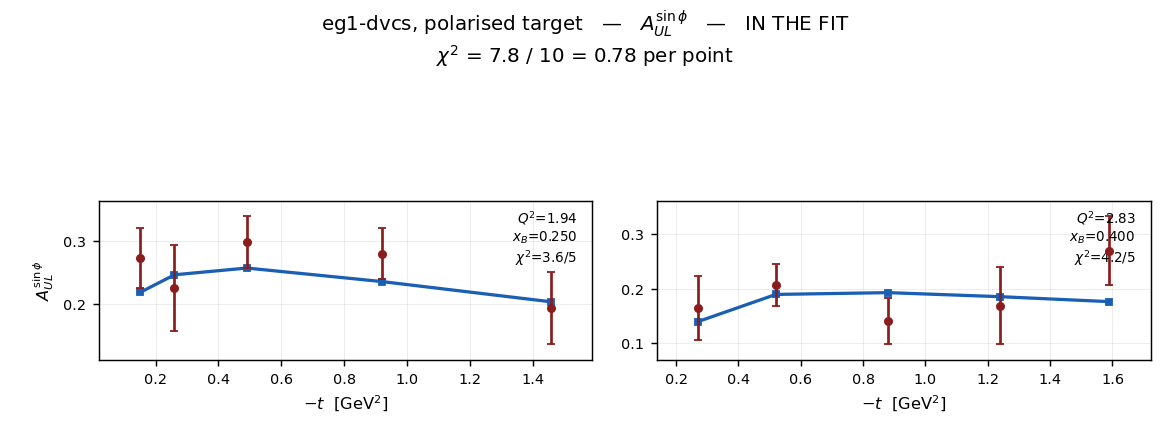
\includegraphics[width=0.72\textwidth]{15_eg1_in_AULsin.png}
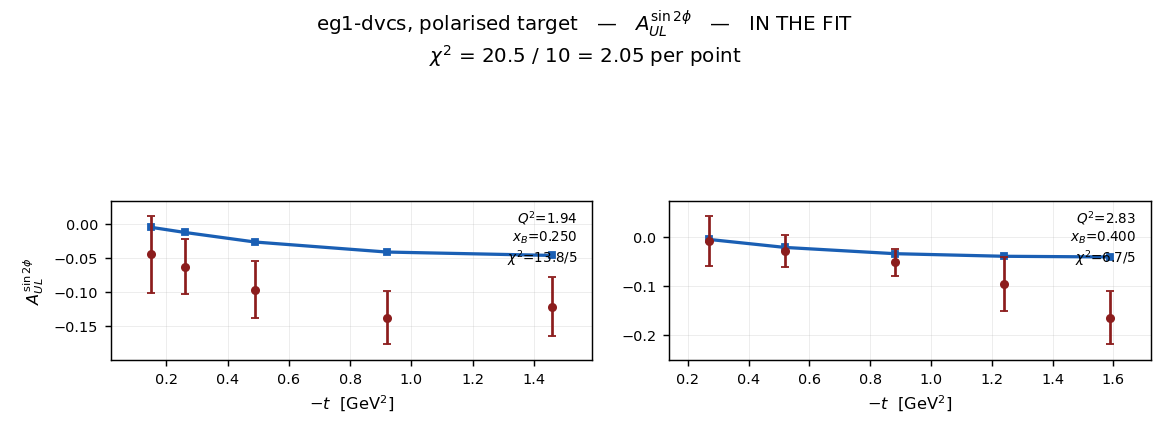
\includegraphics[width=0.72\textwidth]{15_eg1_in_AULsin2.png}
\caption{eg1-dvcs, the $A_{UL}$ moments.}
\end{figure}

\clearpage
\section*{Reproducing this}

Code, data and the full history are at
\url{https://github.com/vkubarovsky/rc_iter1} in the repository
\texttt{pi0eta\_ampmodel\_fit}.  The fit shown is run \texttt{\fittag}; its
parameter vector is \texttt{runs/\fittag/fitpar.npy} and every number in the
tables above is generated from it by \texttt{tex/make\_tables.py}, so nothing
here is transcribed by hand.  The De Masi moments are
\texttt{data/demasi\_moments.txt}, written by \texttt{demasi\_moments.py}, whose
header records the reference model used for the denominator and its md5.  The
recovered Rosenbluth blocks are in \texttt{halla\_rosenbluth.py}.  The remaining
data are \texttt{pi0\_eta\_database.xlsx}; \texttt{export\_db.py --check}
verifies that the CSV cache the fit reads still matches the workbook.

\end{document}
